\apendice{Especificación de diseño}

\section{Introducción}

\section{Diseño de datos}
%Clases
En cuanto al diseño de los datos, se han utilizado las siguientes clases o entidades, que son idénticas tanto en la base de datos, como en el servidor, como en el cliente:
\begin{itemize}
    
    \imagen{./Figuras/Diagramas/paqueteUser.png}{Paquete \texttt{user}}
    \item \textbf{User}: Esta entidad se encarga de almacenar información sobre los usuarios registrados en la base de datos. Dicha entidad consta de los siguientes campos:
    \begin{itemize}
        \item \texttt{emailUser}: Almacena la dirección de correo electrónico del usuario. Es de tipo \texttt{String} o \texttt{VARCHAR(500)}
        \item \texttt{userType}: Indica el tipo de usuario, que puede ser \texttt{ADMIN}, \texttt{DIRECTOR} o \texttt{ORGANIZATION}.Es de tipo \texttt{String} o \texttt{VARCHAR(50)}
        \item \texttt{passwordUser}: Almacena la contraseña del usuario, hasheada en SHA-256. Es de tipo \texttt{String} o \texttt{VARCHAR(500)}.
        \item \texttt{first\_name}: Almacena el nombre del usuario. Es de tipo \texttt{String} o \texttt{VARCHAR(500)}.
        \item \texttt{last\_name}: Almacena el apellido del usuario. Es de tipo \texttt{String} o \texttt{VARCHAR(500)}.
        \item \texttt{idOrganization}: Almacena el identificador de la organización a la
        que pertenece el usuario. Es de tipo \texttt{INT}
        \item \texttt{organizationType}: Indica el tipo de la organización, que
        puede ser "EVALUATED" o "EVALUATOR". Es de tipo \texttt{String} o \texttt{VARCHAR(50)}.
        \item \texttt{illness}: Almacena el tipo de enfermedad relacionada con
        la organización. Es de tipo \texttt{String} o \texttt{VARCHAR(50)}.
        \item \texttt{telephone}: Almacena el número de teléfono del usuario,
        incluyendo el prefijo telefónico de su país. Es de tipo \texttt{String} o
        \texttt{VARCHAR}
        \item \texttt{profilePhoto}: Almacena el nombre del fichero de la fotografía de perfil del usuario, para que pueda acceder Azure Blob Storage. Es de tipo \texttt{String} o \texttt{VARCHAR(MAX)}.
        \item \texttt{isActive}: Esta variable enterna determina si el usuario está o no activo. En caso de que dicho valor sea igual a -1, se trata de un usuario cuya solicitud no ha sido respondida. En caso de que dicho valor sea igual a 0, significa que el usuario está autorizado a registrarse. Si dicho valor es igual a 1, significa que el usuario está activo. Dicho valor es de tipo entero.
        \item \texttt{PRIMARY KEY}: La clave primaria de esta tabla es el campo "emailUser", considerando que no se pueden añadir dos emails iguales.
        \item \texttt{CHECK}: Define una serie de condiciones que los datos deben cumplir para ser válidos, comprobando léxicamente la clave primaria.
      \end{itemize}

      

        \imagen{./Figuras/Diagramas/paqueteOrganization.png}{Paquete \texttt{organization}}
    \item \textbf{Organization}: Esta tabla se encarga de almacenar la información sobre las organizaciones registradas de todos los tipos, utilizando para ello los siguientes campos:
        \begin{itemize}
        \item \texttt{idOrganization}: Almacena el identificador de la organización. Es de tipo \texttt{INT}.
        \item \texttt{orgType}: Indica el tipo de la organización. Es de tipo \texttt{String} o \texttt{VARCHAR(50)}.
        \item \texttt{illness}: Almacena el tipo de enfermedad relacionada con la organización. Es de tipo \texttt{String} o \texttt{VARCHAR(50)}.
        \item \texttt{nameOrg}: Almacena el nombre de la organización.Es de tipo \texttt{String} o \texttt{VARCHAR(500)}.
        \item \texttt{idAddress}: Almacena el identificador de la dirección de la organización.Es de tipo \texttt{INT}.
        \item \texttt{informationSpanish}: Almacena información sobre la organización en español.Es de tipo \texttt{String} o \texttt{VARCHAR(5000)}.
        \item \texttt{informationEnglish}: Almacena información sobre la organización en inglés.Es de tipo \texttt{String} o \texttt{VARCHAR(5000)}.
        \item \texttt{informationFrench}: Almacena información sobre la organización en francés.Es de tipo \texttt{String} o \texttt{VARCHAR(5000)}.
        \item \texttt{informationBasque}: Almacena información sobre la organización en euskera.Es de tipo \texttt{String} o \texttt{VARCHAR(5000)}.
        \item \texttt{informationCatalan}: Almacena información sobre la organización en catalán.Es de tipo \texttt{String} o \texttt{VARCHAR(5000)}.
        \item \texttt{informationDutch}: Almacena información sobre la organización en neerlandés.Es de tipo \texttt{String} o \texttt{VARCHAR(5000)}.
        \item \texttt{informationGalician}: Almacena información sobre la organización en gallego.Es de tipo \texttt{String} o \texttt{VARCHAR(5000)}.
        \item \texttt{informationGerman}: Almacena información sobre la organización en alemán.Es de tipo \texttt{String} o \texttt{VARCHAR(5000)}.
        \item \texttt{informationItalian}: Almacena información sobre la organización en italiano.Es de tipo \texttt{String} o \texttt{VARCHAR(5000)}.
        \item \texttt{informationPortuguese}: Almacena información sobre la organización en portugués.Es de tipo \texttt{String} o \texttt{VARCHAR(5000)}.
        \item \texttt{email}: Almacena la dirección de correo electrónico de la organización.Es de tipo \texttt{String} o \texttt{VARCHAR(500)}.
        \item \texttt{telephone}: Almacena el número de teléfono de la organización.Es de tipo \texttt{String} o \texttt{VARCHAR(50)}.
        \item \texttt{profilePhoto}: Almacena el nombre del fichero de la fotografía de perfil de la organización, para que pueda acceder Azure Blob Storage. Es de tipo \texttt{String} o \texttt{VARCHAR(MAX)}.
        \item \texttt{PRIMARY KEY}: La clave principal de esta tabla está compuesta por los campos \texttt{IdOrganization}, \texttt{orgType} e \texttt{illness}.
        \item \texttt{FOREIGN KEY}: Establece una relación con la entidad \textbf{Address} a través del campo \texttt{idAddress}.
        \end{itemize}
        
\imagen{./Figuras/Diagramas/paqueteIndicator.png}{Paquete \texttt{indicator}}
\imagen{./Figuras/Diagramas/Ambit.png}{Clase \texttt{Ambit}}

    \item \textbf{Ambit}: Esta tabla se encarga de almacenar información sobre los ámbitos almacenados en la base de datos, utilizando para ello los siguientes campos:
        \begin{itemize}
        \item \texttt{idAmbit}: Almacena el identificador del ámbito. Es de tipo \texttt{INT}.
        \item \texttt{descriptionSpanish}: Almacena la descripción en español del ámbito.Es de tipo \texttt{String} o \texttt{VARCHAR(5000)}.
        \item \texttt{descriptionEnglish}: Almacena la descripción en inglés del ámbito.Es de tipo \texttt{String} o \texttt{VARCHAR(5000)}.
        \item \texttt{descriptionFrench}: Almacena la descripción en francés del ámbito.Es de tipo \texttt{String} o \texttt{VARCHAR(5000)}.
        \item \texttt{descriptionBasque}: Almacena la descripción en euskera del ámbito.Es de tipo \texttt{String} o \texttt{VARCHAR(5000)}.
        \item \texttt{descriptionCatalan}: Almacena la descripción en catalán del ámbito.Es de tipo \texttt{String} o \texttt{VARCHAR(5000)}.
        \item \texttt{descriptionDutch}: Almacena la descripción en neerlandés del ámbito.Es de tipo \texttt{String} o \texttt{VARCHAR(5000)}.
        \item \texttt{descriptionGalician}: Almacena la descripción en gallego del ámbito.Es de tipo \texttt{String} o \texttt{VARCHAR(5000)}.
        \item \texttt{descriptionGerman}: Almacena la descripción en alemán del ámbito.Es de tipo \texttt{String} o \texttt{VARCHAR(5000)}.
        \item \texttt{descriptionItalian}: Almacena la descripción en italiano del ámbito.Es de tipo \texttt{String} o \texttt{VARCHAR(5000)}.
        \item \texttt{descriptionPortuguese}: Almacena la descripción en portugués del ámbito.Es de tipo \texttt{String} o \texttt{VARCHAR(5000)}.
        \item \texttt{indicatorType}: Indica el tipo de indicador.Es de tipo \texttt{String} o \texttt{VARCHAR(50)}.
        \item \texttt{PRIMARY KEY}: La clave principal de esta tabla está compuesta por los campos  \texttt{idAmbit} y \texttt{indicatorType}.
        \end{itemize}
    
\imagen{./Figuras/Diagramas/SubAmbit.png}{Clase \texttt{SubAmbit}}

    \item \textbf{SubAmbit}: Esta tabla se encarga de almacenar información sobre los subámbitos (primera división de ámbitos) almacenados en la base de datos, utilizando para ello los siguientes campos:
        \begin{itemize}
        \item \texttt{idSubAmbit}: Almacena el identificador del subámbito. Es de tipo \texttt{INT}.
        \item \texttt{idAmbit}: Almacena el identificador del ámbito. Es de tipo \texttt{INT}.
        \item \texttt{descriptionSpanish}: Almacena la descripción en español del subámbito.Es de tipo \texttt{String} o \texttt{VARCHAR(5000)}.
        \item \texttt{descriptionEnglish}: Almacena la descripción en inglés del subámbito.Es de tipo \texttt{String} o \texttt{VARCHAR(5000)}.
        \item \texttt{descriptionFrench}: Almacena la descripción en francés del subámbito.Es de tipo \texttt{String} o \texttt{VARCHAR(5000)}.
        \item \texttt{descriptionBasque}: Almacena la descripción en euskera del subámbito.Es de tipo \texttt{String} o \texttt{VARCHAR(5000)}.
        \item \texttt{descriptionCatalan}: Almacena la descripción en catalán del subámbito.Es de tipo \texttt{String} o \texttt{VARCHAR(5000)}.
        \item \texttt{descriptionDutch}: Almacena la descripción en neerlandés del subámbito.Es de tipo \texttt{String} o \texttt{VARCHAR(5000)}.
        \item \texttt{descriptionGalician}: Almacena la descripción en gallego del subámbito.Es de tipo \texttt{String} o \texttt{VARCHAR(5000)}.
        \item \texttt{descriptionGerman}: Almacena la descripción en alemán del subámbito.Es de tipo \texttt{String} o \texttt{VARCHAR(5000)}.
        \item \texttt{descriptionItalian}: Almacena la descripción en italiano del subámbito.Es de tipo \texttt{String} o \texttt{VARCHAR(5000)}.
        \item \texttt{descriptionPortuguese}: Almacena la descripción en portugués del subámbito.Es de tipo \texttt{String} o \texttt{VARCHAR(5000)}.
        \item \texttt{indicatorType}: Indica el tipo de indicador.Es de tipo \texttt{String} o \texttt{VARCHAR(50)}.
        \item \texttt{PRIMARY KEY}: La clave principal de esta tabla está compuesta por los campos \texttt{idSubAmbit}, \texttt{idAmbit}, \texttt{indicatorType}.
        \item \texttt{FOREIGN KEY}: Establece una relación con la entidad \textbf{Ambit} a través de los campos \texttt{indicatorType}, \texttt{idSubAmbit} e \texttt{idAmbit}.
        \end{itemize}

\imagen{./Figuras/Diagramas/SubSubAmbit.png}{Clase \texttt{SubSubAmbit}}


    \item \textbf{SubSubAmbit}: Esta tabla se encarga de almacenar información sobre los subsubámbitos (segunda división de ámbitos) almacenados en la base de datos, utilizando para ello los siguientes campos:
        \begin{itemize}
        \item \texttt{idSubSubAmbit}: Almacena el identificador del subsubámbito. Es de tipo \texttt{INT}.
        \item \texttt{idSubAmbit}: Almacena el identificador del subámbito. Es de tipo \texttt{INT}.
        \item \texttt{idAmbit}: Almacena el identificador del ámbito. Es de tipo \texttt{INT}.
        \item \texttt{descriptionSpanish}: Almacena la descripción en español del subsubámbito.Es de tipo \texttt{String} o \texttt{VARCHAR(5000)}.
        \item \texttt{descriptionEnglish}: Almacena la descripción en inglés del subsubámbito.Es de tipo \texttt{String} o \texttt{VARCHAR(5000)}.
        \item \texttt{descriptionFrench}: Almacena la descripción en francés del subsubámbito.Es de tipo \texttt{String} o \texttt{VARCHAR(5000)}.
        \item \texttt{descriptionBasque}: Almacena la descripción en euskera del subsubámbito.Es de tipo \texttt{String} o \texttt{VARCHAR(5000)}.
        \item \texttt{descriptionCatalan}: Almacena la descripción en catalán del subsubámbito.Es de tipo \texttt{String} o \texttt{VARCHAR(5000)}.
        \item \texttt{descriptionDutch}: Almacena la descripción en neerlandés del subsubámbito.Es de tipo \texttt{String} o \texttt{VARCHAR(5000)}.
        \item \texttt{descriptionGalician}: Almacena la descripción en gallego del subsubámbito.Es de tipo \texttt{String} o \texttt{VARCHAR(5000)}.
        \item \texttt{descriptionGerman}: Almacena la descripción en alemán del subsubámbito.Es de tipo \texttt{String} o \texttt{VARCHAR(5000)}.
        \item \texttt{descriptionItalian}: Almacena la descripción en italiano del subsubámbito.Es de tipo \texttt{String} o \texttt{VARCHAR(5000)}.
        \item \texttt{descriptionPortuguese}: Almacena la descripción en portugués del subsubámbito.Es de tipo \texttt{String} o \texttt{VARCHAR(5000)}.
        \item \texttt{indicatorType}: Indica el tipo de indicador.Es de tipo \texttt{String} o \texttt{VARCHAR(50)}.
        \item \texttt{PRIMARY KEY}: La clave principal de esta tabla está compuesta por los campos \texttt{idSubSubAmbit}, \texttt{idSubAmbit}, \texttt{idAmbit}, \texttt{indicatorType}.
        \item \texttt{FOREIGN KEY}: Establece una relación con la entidad \textbf{SubAmbit} a través de los campos \texttt{indicatorType}, \texttt{idSubAmbit} e \texttt{idAmbit}.
        \end{itemize}

\imagen{./Figuras/Diagramas/Indicator.png}{Clase \texttt{Indicator}}

    \item \textbf{Indicator}: Esta tabla se encarga de almacenar información sobre los indicadores almacenados en la base de datos, utilizando para ello los siguientes campos:
        \begin{itemize}
        \item \texttt{idIndicator}: Almacena el identificador del indicador. Es de tipo \texttt{INT}.
        \item \texttt{indicatorType}: Indica el tipo de indicador.Es de tipo \texttt{String} o \texttt{VARCHAR(50)}.
        \item \texttt{idSubSubAmbit}: Almacena el identificador del subsubámbito. Es de tipo \texttt{INT}.
        \item \texttt{idSubAmbit}: Almacena el identificador del subámbito. Es de tipo \texttt{INT}.
        \item \texttt{idAmbit}: Almacena el identificador del ámbito. Es de tipo \texttt{INT}.
        \item \texttt{descriptionSpanish}: Almacena la descripción en español del indicador.Es de tipo \texttt{String} o \texttt{VARCHAR(5000)}.
        \item \texttt{descriptionEnglish}: Almacena la descripción en inglés del indicador.Es de tipo \texttt{String} o \texttt{VARCHAR(5000)}.
        \item \texttt{descriptionFrench}: Almacena la descripción en francés del indicador.Es de tipo \texttt{String} o \texttt{VARCHAR(5000)}.
        \item \texttt{descriptionBasque}: Almacena la descripción en euskera del indicador.Es de tipo \texttt{String} o \texttt{VARCHAR(5000)}.
        \item \texttt{descriptionCatalan}: Almacena la descripción en catalán del indicador.Es de tipo \texttt{String} o \texttt{VARCHAR(5000)}.
        \item \texttt{descriptionDutch}: Almacena la descripción en neerlandés del indicador.Es de tipo \texttt{String} o \texttt{VARCHAR(5000)}.
        \item \texttt{descriptionGalician}: Almacena la descripción en gallego del indicador.Es de tipo \texttt{String} o \texttt{VARCHAR(5000)}.
        \item \texttt{descriptionGerman}: Almacena la descripción en alemán del indicador.Es de tipo \texttt{String} o \texttt{VARCHAR(5000)}.
        \item \texttt{descriptionItalian}: Almacena la descripción en italiano del indicador.Es de tipo \texttt{String} o \texttt{VARCHAR(5000)}.
        \item \texttt{descriptionPortuguese}: Almacena la descripción en portugués del indicador.Es de tipo \texttt{String} o \texttt{VARCHAR(5000)}.
        \item \texttt{indicatorVersion}: Almacena la versión del indicador. Es de tipo \texttt{INT}.
        \item \texttt{isActive}: Indica si el indicador está en uso o no. Es de tipo \texttt{INT}.
        \item \texttt{evaluationType}: Almacena si el indicador pertenece a la evaluación completa o a la evaluación simple. Es de tipo \texttt{String} o \texttt{VARCHAR(50)}.
        \item \texttt{indicatorPriority}: Almacena la prioridad del indicador. Es de tipo \texttt{String} o \texttt{VARCHAR(50)}.
        \item \texttt{PRIMARY KEY}: La clave principal de esta tabla está compuesta por los campos \texttt{idIndicator}, \texttt{indicatorType}, \texttt{idSubSubAmbit}, \texttt{idSubAmbit}, \texttt{idAmbit}, \texttt{indicatorVersion} y \texttt{evaluationType}.
        \item \texttt{FOREIGN KEY}: Establece una relación con la entidad \textbf{SubSubAmbit} a través de los campos \texttt{indicatorType}, \texttt{idSubSubAmbit}, \texttt{idSubAmbit}, \texttt{idAmbit} e \texttt{indicatorType}.
        \end{itemize}

\imagen{./Figuras/Diagramas/Evidence.png}{Clase \texttt{Evidence}}

    \item \textbf{Evidence}: Esta entidad se encarga de almacenar información sobre todas las evidencias de cada uno de los indicadores, utilizando para ello los siguientes campos:
        \begin{itemize}
        \item \texttt{idEvidence}: Almacena el identificador de la evidencia. Es de tipo \texttt{INT}.
        \item \texttt{idIndicator}: Almacena el identificador del indicador al que pertenece la evidencia. Es de tipo \texttt{INT}.
        \item \texttt{indicatorType}: Indica el tipo de indicador.Es de tipo \texttt{String} o \texttt{VARCHAR(50)}.
        \item \texttt{idSubSubAmbit}: Almacena el identificador del subsubámbito. Es de tipo \texttt{INT}.
        \item \texttt{idSubAmbit}: Almacena el identificador del subámbito. Es de tipo \texttt{INT}.
        \item \texttt{idAmbit}: Almacena el identificador del ámbito. Es de tipo \texttt{INT}.
        \item \texttt{indicatorVersion}: Almacena la versión del indicador. Es de tipo \texttt{INT}.
        \item \texttt{descriptionSpanish}: Almacena la descripción en español de la evidencia.Es de tipo \texttt{String} o \texttt{VARCHAR(5000)}.
        \item \texttt{descriptionEnglish}: Almacena la descripción en inglés de la evidencia.Es de tipo \texttt{String} o \texttt{VARCHAR(5000)}.
        \item \texttt{descriptionFrench}: Almacena la descripción en francés de la evidencia.Es de tipo \texttt{String} o \texttt{VARCHAR(5000)}.
        \item \texttt{descriptionBasque}: Almacena la descripción en euskera de la evidencia.Es de tipo \texttt{String} o \texttt{VARCHAR(5000)}.
        \item \texttt{descriptionCatalan}: Almacena la descripción en catalán de la evidencia.Es de tipo \texttt{String} o \texttt{VARCHAR(5000)}.
        \item \texttt{descriptionDutch}: Almacena la descripción en neerlandés de la evidencia.Es de tipo \texttt{String} o \texttt{VARCHAR(5000)}.
        \item \texttt{descriptionGalician}: Almacena la descripción en gallego de la evidencia.Es de tipo \texttt{String} o \texttt{VARCHAR(5000)}.
        \item \texttt{descriptionGerman}: Almacena la descripción en alemán de la evidencia.Es de tipo \texttt{String} o \texttt{VARCHAR(5000)}.
        \item \texttt{descriptionItalian}: Almacena la descripción en italiano de la evidencia.Es de tipo \texttt{String} o \texttt{VARCHAR(5000)}.
        \item \texttt{descriptionPortuguese}: Almacena la descripción en portugués de la evidencia.Es de tipo \texttt{String} o \texttt{VARCHAR(5000)}.
        \item \texttt{evidenceValue}: Almacena el valor de la evidencia. Es de tipo \texttt{INT}.
        \item \texttt{evaluationType}: Almacena si la evidencia pertenece a la evaluación completa o a la evaluación simple. Es de tipo \texttt{String} o \texttt{VARCHAR(50)}.
        \item \texttt{PRIMARY KEY}: La clave principal de esta tabla está compuesta por los campos \texttt{idEvidence}, \texttt{idIndicator}, \texttt{indicatorType}, \texttt{idSubSubAmbit}, \texttt{idSubAmbit}, \texttt{idAmbit}, \texttt{indicatorVersion} y \texttt{evaluationType}.
        \item \texttt{FOREIGN KEY}: Establece una relación con la entidad \textbf{Indicator} a través de los campos \texttt{idIndicator}, \texttt{indicatorType}, \texttt{idSubSubAmbit}, \texttt{idSubAmbit}, \texttt{idAmbit}, \texttt{indicatorVersion} y \texttt{evaluationType}.
        \end{itemize}


\begin{figure}[H]
    \centering
    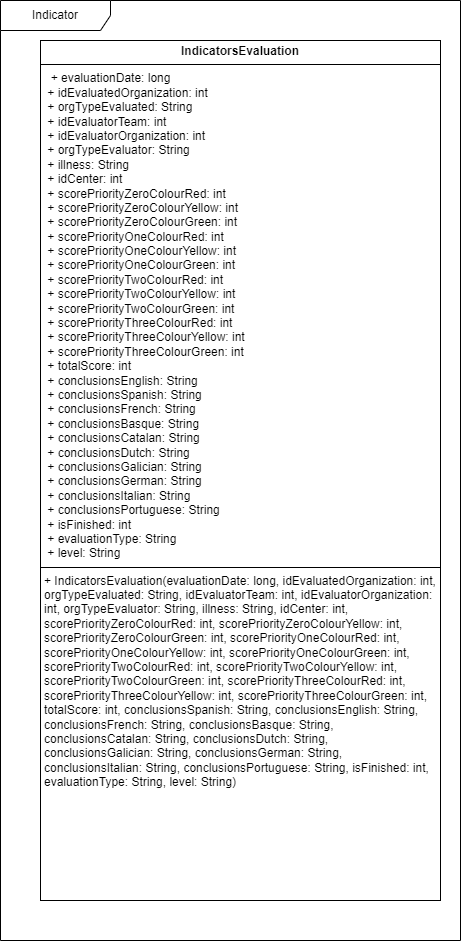
\includegraphics[width=0.6\textwidth]{./Figuras/Diagramas/IndicatorsEvaluation.png}
    \caption{Clase \texttt{IndicatorsEvaluation}}\label{fig:./Figuras/Diagramas/IndicatorsEvaluation.png}
\end{figure}
        
   
    \item \textbf{IndicatorsEvaluation}: Esta entidad se encarga de almacenar la información sobre los diferentes test de indicadores, utilizando para ello los siguientes campos:
    \begin{itemize}
      \item \texttt{evaluationDate}: Almacena la fecha de evaluación de los indicadores.Es de tipo \texttt{long} o \texttt{BIGINT}.
      \item \texttt{idEvaluatedOrganization}: Almacena el identificador de la organización evaluada.Es de tipo \texttt{INT}.
      \item \texttt{orgTypeEvaluated}: Indica el tipo de la organización evaluada.Es de tipo \texttt{String} o de tipo
      \item \texttt{idEvaluatorTeam}: Almacena el identificador del equipo evaluador que realizó la evaluación.Es de tipo \texttt{INT}.
      \item \texttt{idEvaluatorOrganization}: Almacena el identificador de la organización a la que pertenece el equipo evaluador.Es de tipo \texttt{INT}.
      \item \texttt{orgTypeEvaluator}: Indica el tipo de la organización evaluadora.
      \item \texttt{idCenter}: Almacena el identificador del centro.Es de tipo \texttt{INT}.
      \item \texttt{illness}: Almacena el tipo de enfermedad relacionada con la organización evaluada.
      \item \texttt{totalScore}: Almacena la puntuación total del test de indicadores.Es de tipo \texttt{INT}.
      \item \texttt{conclusionsSpanish}: Almacena las conclusiones del test de indicadores en español. Es de tipo \texttt{String} o \texttt{VARCHAR(5000)}.
      \item \texttt{conclusionsEnglish}: Almacena las conclusiones del test de indicadores en inglés. Es de tipo \texttt{String} o \texttt{VARCHAR(5000)}.
      \item \texttt{conclusionsFrench}: Almacena las conclusiones del test de indicadores en francés. Es de tipo \texttt{String} o \texttt{VARCHAR(5000)}.
      \item \texttt{conclusionsBasque}: Almacena las conclusiones del test de indicadores en euskera. Es de tipo \texttt{String} o \texttt{VARCHAR(5000)}.
      \item \texttt{conclusionsCatalan}: Almacena las conclusiones del test de indicadores en catalán. Es de tipo \texttt{String} o \texttt{VARCHAR(5000)}.
      \item \texttt{conclusionsDutch}: Almacena las conclusiones del test de indicadores en neerlandés. Es de tipo \texttt{String} o \texttt{VARCHAR(5000)}.
      \item \texttt{conclusionsGalician}: Almacena las conclusiones del test de indicadores en gallego. Es de tipo \texttt{String} o \texttt{VARCHAR(5000)}.
      \item \texttt{conclusionsGerman}: Almacena las conclusiones del test de indicadores en alemán. Es de tipo \texttt{String} o \texttt{VARCHAR(5000)}.
      \item \texttt{conclusionsItalian}: Almacena las conclusiones del test de indicadores en italiano. Es de tipo \texttt{String} o \texttt{VARCHAR(5000)}.
      \item \texttt{conclusionsPortuguese}: Almacena las conclusiones del test de indicadores en portugués. Es de tipo \texttt{String} o \texttt{VARCHAR(5000)}.
      \item \texttt{isFinished}: Almacena si el test de indicadores ha finalizado (1) o no ha finalizado (0). Es de tipo \texttt{INT}.
      \item \texttt{evaluationType}: Almacena si el indicador pertenece a la evaluación completa o a la evaluación simple. Es de tipo \texttt{String} o \texttt{VARCHAR(50)}.
      \item \texttt{scorePriorityZeroColourRed}: Almacena el puntaje para los indicadores de estado \texttt{IN\_START} el interés \texttt{LOW\_INTEREST}.Es de tipo \texttt{INT}.
      \item \texttt{scorePriorityZeroColourYellow}: Almacena el puntaje para los indicadores de estado \texttt{IN\_PROCESS} el interés \texttt{LOW\_INTEREST}.Es de tipo \texttt{INT}.
      \item \texttt{scorePriorityZeroColourGreen}: Almacena el puntaje para los indicadores de estado \texttt{REACHED} el interés \texttt{LOW\_INTEREST}.Es de tipo \texttt{INT}.
      \item \texttt{scorePriorityOneColourRed}: Almacena el puntaje para los indicadores de estado \texttt{IN\_START} el interés \texttt{MEDIUM\_INTEREST}.Es de tipo \texttt{INT}.
      \item \texttt{scorePriorityOneColourYellow}: Almacena el puntaje para los indicadores de estado \texttt{IN\_PROCESS} el interés \texttt{MEDIUM\_INTEREST}.Es de tipo \texttt{INT}.
      \item \texttt{scorePriorityOneColourGreen}: Almacena el puntaje para los indicadores de estado \texttt{REACHED} el interés \texttt{MEDIUM\_INTEREST}.Es de tipo \texttt{INT}.
      \item \texttt{scorePriorityTwoColourRed}: Almacena el puntaje para los indicadores de estado \texttt{IN\_START} el interés \texttt{HIGH\_INTEREST}.Es de tipo \texttt{INT}.
      \item \texttt{scorePriorityTwoColourYellow}: Almacena el puntaje para los indicadores de estado \texttt{IN\_PROCESS} el interés \texttt{HIGH\_INTEREST}.Es de tipo \texttt{INT}.
      \item \texttt{scorePriorityTwoColourGreen}: Almacena el puntaje para los indicadores de estado \texttt{REACHED} el interés \texttt{HIGH\_INTEREST}.Es de tipo \texttt{INT}.
      \item \texttt{scorePriorityThreeColourRed}: Almacena el puntaje para los indicadores de estado \texttt{IN\_START} el interés \texttt{FUNDAMENTAL\_INTEREST}.Es de tipo \texttt{INT}.
      \item \texttt{scorePriorityThreeColourYellow}: Almacena el puntaje para los indicadores de estado \texttt{IN\_PROCESS} el interés \texttt{FUNDAMENTAL\_INTEREST}.Es de tipo \texttt{INT}.
      \item \texttt{scorePriorityThreeColourGreen}: Almacena el puntaje para los indicadores de estado \texttt{REACHED} el interés \texttt{FUNDAMENTAL\_INTEREST}.Es de tipo \texttt{INT}.
      \item \texttt{level}: Almacena el nivel del indicador, obtenido del sistema experto. El valor puede ser \texttt{IN\_START}, \texttt{IN\_PROCESS} o \texttt{REACHED}. Es de tipo \texttt{String} o \texttt{VARCHAR(50)}.
      \item \texttt{PRIMARY KEY}: La clave principal de esta tabla está compuesta por los campos \texttt{evaluationDate}, \texttt{idEvaluatorTeam}, \texttt{idEvaluatorOrganization}, \texttt{orgTypeEvaluator}, \texttt{idEvaluatedOrganization}, \texttt{orgTypeEvaluated}, \texttt{idCenter}, \texttt{illness} y \texttt{evaluationType}.
      \item \texttt{FOREIGN KEY}: Establece una relación con la entidad \textbf{EvaluatorTeam} a través de los campos \texttt{idEvaluatorTeam}, \texttt{idEvaluatorOrganization}, \texttt{orgTypeEvaluator}, \texttt{idEvaluatedOrganization}, \texttt{orgTypeEvaluated}, \texttt{idCenter} e \texttt{illness}.
    \end{itemize}
    



    \begin{figure}[H]
		\centering
		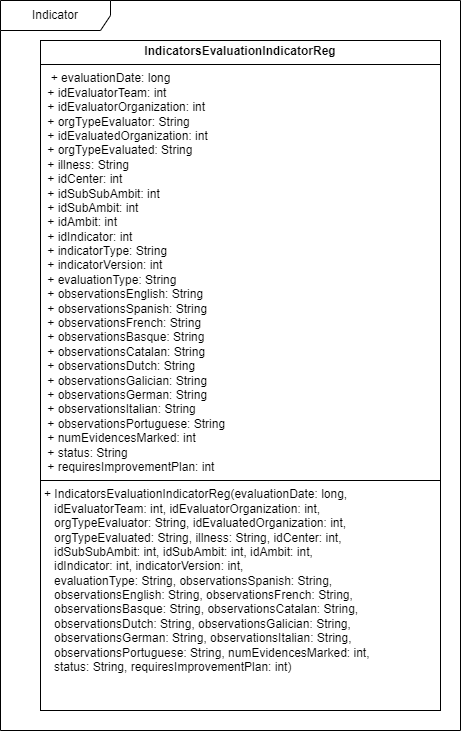
\includegraphics[width=0.6\textwidth]{./Figuras/Diagramas/IndicatorsEvaluationIndicatorReg.png}
		\caption{Clase \texttt{IndicatorsEvaluationIndicatorReg}}\label{fig:./Figuras/Diagramas/IndicatorsEvaluationIndicatorReg.png}
	\end{figure}

    \item \textbf{IndicatorsEvaluationIndicatorReg}: Esta entidad se encarga de almacenar los registros de evidencias (para evaluaciones completas) de cada uno de los test de indicadores realizados, existiendo uno para cada evidencia rellenada, utilizando para ello los siguientes campos:
    \begin{itemize}
      \item \texttt{evaluationDate}: Almacena la fecha de la evaluación de los indicadores.
      \item \texttt{idEvaluatedOrganization}: Almacena el identificador de la organización evaluada.Es de tipo \texttt{INT}.
      \item \texttt{orgTypeEvaluated}: Indica el tipo de la organización evaluada.
      \item \texttt{idEvaluatorTeam}: Almacena el identificador del equipo evaluador que realizó la evaluación.Es de tipo \texttt{INT}.
      \item \texttt{idEvaluatorOrganization}: Almacena el identificador de la organización a la que pertenece el equipo evaluador.Es de tipo \texttt{INT}.
      \item \texttt{orgTypeEvaluator}: Indica el tipo de la organización evaluadora.
      \item \texttt{illness}: Almacena el tipo de enfermedad relacionada con la organización evaluada.
      \item \texttt{idCenter}: Almacena el identificador del centro.Es de tipo \texttt{INT}.
      \item \texttt{idIndicator}: Almacena el identificador del indicador evaluado. Es de tipo \texttt{INT}.
      \item \texttt{indicatorType}: Indica el tipo de indicador.Es de tipo \texttt{String} o \texttt{VARCHAR(50)}.
      \item \texttt{idSubSubAmbit}: Almacena el identificador del subsubámbito. Es de tipo \texttt{INT}.
      \item \texttt{idSubAmbit}: Almacena el identificador del subámbito. Es de tipo \texttt{INT}.
      \item \texttt{idAmbit}: Almacena el identificador del ámbito. Es de tipo \texttt{INT}.
      \item \texttt{indicatorVersion}: Almacena la versión del indicador evaluado. Es de tipo \texttt{INT}.
      \item \texttt{evaluationType}: Almacena si el indicador pertenece a la evaluación completa o a la evaluación simple. Es de tipo \texttt{String} o \texttt{VARCHAR(50)}.
      \item \texttt{observationsSpanish}: Almacena las observaciones del registro en español. Es de tipo \texttt{String} o \texttt{VARCHAR(MAX)}.
        \item \texttt{observationsEnglish}: Almacena las observaciones del registro en inglés. Es de tipo \texttt{String} o \texttt{VARCHAR(MAX)}.
        \item \texttt{observationsFrench}: Almacena las observaciones del registro en francés. Es de tipo \texttt{String} o \texttt{VARCHAR(MAX)}.
        \item \texttt{observationsBasque}: Almacena las observaciones del registro en euskera. Es de tipo \texttt{String} o \texttt{VARCHAR(MAX)}.
        \item \texttt{observationsCatalan}: Almacena las observaciones del registro en catalán. Es de tipo \texttt{String} o \texttt{VARCHAR(MAX)}.
        \item \texttt{observationsDutch}: Almacena las observaciones del registro en neerlandés. Es de tipo \texttt{String} o \texttt{VARCHAR(MAX)}.
        \item \texttt{observationsGalician}: Almacena las observaciones del registro en gallego. Es de tipo \texttt{String} o \texttt{VARCHAR(MAX)}.
        \item \texttt{observationsGerman}: Almacena las observaciones del registro en alemán. Es de tipo \texttt{String} o \texttt{VARCHAR(MAX)}.
        \item \texttt{observationsItalian}: Almacena las observaciones del registro en italiano. Es de tipo \texttt{String} o \texttt{VARCHAR(MAX)}.
        \item \texttt{observationsPortuguese}: Almacena las observaciones del registro en portugués. Es de tipo \texttt{String} o \texttt{VARCHAR(MAX)}.
      \item \texttt{numEvidencesMarked}: Almacena el número de evidencias marcadas para ese indicador. Es de tipo \texttt{INT}.
      \item \texttt{status}: Almacena el estado del indicador, que puede ser \texttt{IN\_START}, \texttt{IN\_PROCESS} o \texttt{REACHED}, valores obtenidos por el sistema experto a partir de \texttt{numEvidencesMarked}. Es de tipo \texttt{String} o \texttt{VARCHAR(50)}
      \item \texttt{requiresImprovementPlan}: Almacena si el indicador requiere estar en el plan de mejora (1) o no (0), se obtiene a partir del sistema experto con el valor de \texttt{status}. Es de tipo \texttt{INT}.  
      \item \texttt{PRIMARY KEY}: La clave principal de esta tabla está compuesta por los campos \texttt{evaluationDate}, \texttt{idEvaluatorTeam}, \texttt{idEvaluatorOrganization}, \texttt{orgTypeEvaluator}, \texttt{idEvaluatedOrganization}, \texttt{orgTypeEvaluated}, \texttt{idCenter}, \texttt{illness}, \texttt{idIndicator}, \texttt{indicatorType}, \texttt{idSubSubAmbit}, \texttt{idSubAmbit}, \texttt{idAmbit}, \texttt{indicatorVersion} y \texttt{evaluationType}.
      \item \texttt{FOREIGN KEY}: Establece una relación con la entidad \textbf{Indicator} a través de los campos \texttt{idIndicator}, \texttt{indicatorType}, \texttt{idSubSubAmbit}, \texttt{idSubAmbit}, \texttt{idAmbit}, \texttt{indicatorVersion} y \texttt{evaluationType}.
      \item \texttt{FOREIGN KEY}: Establece una relación con la entidad \textbf{IndicatorsEvaluation} a través de los campos \texttt{evaluationDate}, \texttt{idEvaluatedOrganization}, \texttt{orgTypeEvaluated}, \texttt{illness}, \texttt{indicatorVersion} y \texttt{evaluationType}.
    \end{itemize}
    

    \begin{figure}[H]
        \centering
        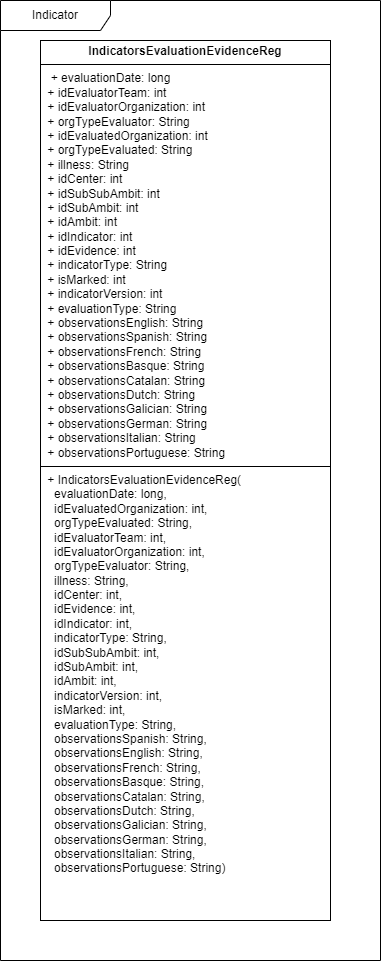
\includegraphics[width=0.6\textwidth]{./Figuras/Diagramas/IndicatorsEvaluationEvidenceReg.png}
        \caption{Clase \texttt{IndicatorsEvaluationEvidenceReg}}\label{fig:./Figuras/Diagramas/IndicatorsEvaluationEvidenceReg.png}
    \end{figure}

    \item \textbf{IndicatorsEvaluationEvidenceReg}: Esta entidad se encarga de almacenar los registros de evidencias (para evaluaciones completas) de cada uno de los test de indicadores realizados, existiendo uno para cada evidencia rellenada, utilizando para ello los siguientes campos:
    \begin{itemize}
      \item \texttt{evaluationDate}: Almacena la fecha de la evaluación de los indicadores.
      \item \texttt{idEvaluatedOrganization}: Almacena el identificador de la organización evaluada.Es de tipo \texttt{INT}.
      \item \texttt{orgTypeEvaluated}: Indica el tipo de la organización evaluada.
      \item \texttt{idEvaluatorTeam}: Almacena el identificador del equipo evaluador que realizó la evaluación.Es de tipo \texttt{INT}.
      \item \texttt{idEvaluatorOrganization}: Almacena el identificador de la organización a la que pertenece el equipo evaluador.Es de tipo \texttt{INT}.
      \item \texttt{orgTypeEvaluator}: Indica el tipo de la organización evaluadora.
      \item \texttt{illness}: Almacena el tipo de enfermedad relacionada con la organización evaluada.
      \item \texttt{idCenter}: Almacena el identificador del centro.Es de tipo \texttt{INT}.
      \item \texttt{idEvidence}: Almacena el identificador de la evidencia relacionada con el indicador.Es de tipo \texttt{INT}.
      \item \texttt{idIndicator}: Almacena el identificador del indicador evaluado. Es de tipo \texttt{INT}.
      \item \texttt{indicatorType}: Indica el tipo de indicador.Es de tipo \texttt{String} o \texttt{VARCHAR(50)}.
      \item \texttt{idSubSubAmbit}: Almacena el identificador del subsubámbito. Es de tipo \texttt{INT}.
      \item \texttt{idSubAmbit}: Almacena el identificador del subámbito. Es de tipo \texttt{INT}.
      \item \texttt{idAmbit}: Almacena el identificador del ámbito. Es de tipo \texttt{INT}.
      \item \texttt{indicatorVersion}: Almacena la versión del indicador evaluado. Es de tipo \texttt{INT}.
      \item \texttt{isMarked}: Es un campo entero no nulo que indica si el indicador está marcado o no. Solo puede tener valores 0 o 1, lo que se verifica con una restricción \texttt{CHECK}.Es de tipo \texttt{INT}.
      \item \texttt{evaluationType}: Almacena si el indicador pertenece a la evaluación completa o a la evaluación simple. Es de tipo \texttt{String} o \texttt{VARCHAR(50)}.
      \item \texttt{observationsSpanish}: Almacena las observaciones del registro en español. Es de tipo \texttt{String} o \texttt{VARCHAR(MAX)}.
        \item \texttt{observationsEnglish}: Almacena las observaciones del registro en inglés. Es de tipo \texttt{String} o \texttt{VARCHAR(MAX)}.
        \item \texttt{observationsFrench}: Almacena las observaciones del registro en francés. Es de tipo \texttt{String} o \texttt{VARCHAR(MAX)}.
        \item \texttt{observationsBasque}: Almacena las observaciones del registro en euskera. Es de tipo \texttt{String} o \texttt{VARCHAR(MAX)}.
        \item \texttt{observationsCatalan}: Almacena las observaciones del registro en catalán. Es de tipo \texttt{String} o \texttt{VARCHAR(MAX)}.
        \item \texttt{observationsDutch}: Almacena las observaciones del registro en neerlandés. Es de tipo \texttt{String} o \texttt{VARCHAR(MAX)}.
        \item \texttt{observationsGalician}: Almacena las observaciones del registro en gallego. Es de tipo \texttt{String} o \texttt{VARCHAR(MAX)}.
        \item \texttt{observationsGerman}: Almacena las observaciones del registro en alemán. Es de tipo \texttt{String} o \texttt{VARCHAR(MAX)}.
        \item \texttt{observationsItalian}: Almacena las observaciones del registro en italiano. Es de tipo \texttt{String} o \texttt{VARCHAR(MAX)}.
        \item \texttt{observationsPortuguese}: Almacena las observaciones del registro en portugués. Es de tipo \texttt{String} o \texttt{VARCHAR(MAX)}.
      \item \texttt{PRIMARY KEY}: La clave principal de esta tabla está compuesta por los campos \texttt{evaluationDate}, \texttt{idEvaluatorTeam}, \texttt{idEvaluatorOrganization}, \texttt{orgTypeEvaluator}, \texttt{idEvaluatedOrganization}, \texttt{orgTypeEvaluated}, \texttt{idCenter}, \texttt{illness}, \texttt{idEvidence}, \texttt{idIndicator}, \texttt{indicatorType}, \texttt{idSubSubAmbit}, \texttt{idSubAmbit}, \texttt{idAmbit}, \texttt{indicatorVersion} y \texttt{evaluationType}.
      \item \texttt{FOREIGN KEY}: Establece una relación con la entidad \textbf{Evidence} a través de los campos \texttt{idEvidence}, \texttt{idIndicator}, \texttt{indicatorType}, \texttt{idSubSubAmbit}, \texttt{idSubAmbit}, \texttt{idAmbit}, \texttt{indicatorVersion} y \texttt{evaluationType}.
      \item \texttt{FOREIGN KEY}: Establece una relación con la entidad \textbf{IndicatorsEvaluation} a través de los campos \texttt{evaluationDate}, \texttt{idEvaluatedOrganization}, \texttt{orgTypeEvaluated}, \texttt{illness}, \texttt{indicatorVersion} y \texttt{evaluationType}.
    \end{itemize}


    \begin{figure}[H]
        \centering
        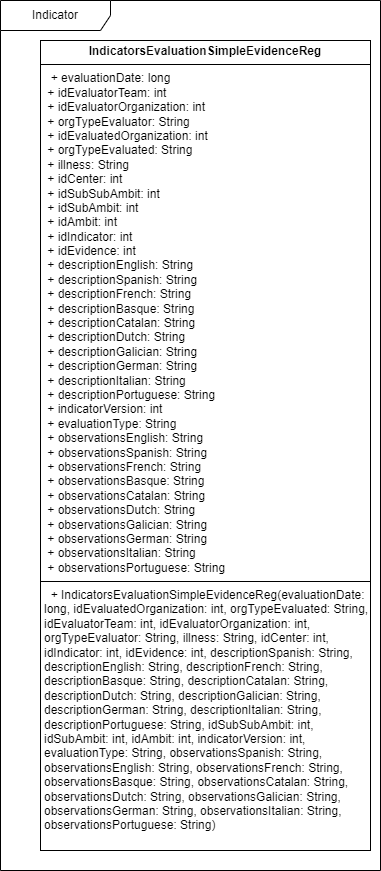
\includegraphics[width=0.6\textwidth]{./Figuras/Diagramas/IndicatorsEvaluationSimpleEvidenceReg.png}
        \caption{Clase \texttt{IndicatorsEvaluationSimpleEvidenceReg}}\label{fig:./Figuras/Diagramas/IndicatorsEvaluationSimpleEvidenceReg.png}
    \end{figure}
    
    
    \item \textbf{IndicatorsEvaluationSimpleEvidenceReg}: Esta entidad se encarga de almacenar los registros de evidencias (para evaluaciones simples) de cada uno de los test de indicadores realizados, existiendo uno para cada evidencia rellenada, utilizando para ello los siguientes campos:
    \begin{itemize}
      \item \texttt{evaluationDate}: Almacena la fecha de la evaluación de los indicadores.
      \item \texttt{idEvaluatedOrganization}: Almacena el identificador de la organización evaluada.Es de tipo \texttt{INT}.
      \item \texttt{orgTypeEvaluated}: Indica el tipo de la organización evaluada.
      \item \texttt{idEvaluatorTeam}: Almacena el identificador del equipo evaluador que realizó la evaluación.Es de tipo \texttt{INT}.
      \item \texttt{idEvaluatorOrganization}: Almacena el identificador de la organización a la que pertenece el equipo evaluador.Es de tipo \texttt{INT}.
      \item \texttt{orgTypeEvaluator}: Indica el tipo de la organización evaluadora.
      \item \texttt{illness}: Almacena el tipo de enfermedad relacionada con la organización evaluada.
      \item \texttt{idCenter}: Almacena el identificador del centro.Es de tipo \texttt{INT}.
      \item \texttt{idIndicator}: Almacena el identificador del indicador evaluado. Es de tipo \texttt{INT}.
      \item \texttt{idEvidence}: Almacena el identificador de la evidencia relacionada con el indicador.Es de tipo \texttt{INT}.
      \item \texttt{descriptionSpanish}: Almacena las descripción de la evidencia en español. Es de tipo \texttt{String} o \texttt{VARCHAR(MAX)}.
        \item \texttt{descriptionEnglish}: Almacena las descripción de la evidencia en inglés. Es de tipo \texttt{String} o \texttt{VARCHAR(MAX)}.
        \item \texttt{descriptionFrench}: Almacena las descripción de la evidencia en francés. Es de tipo \texttt{String} o \texttt{VARCHAR(MAX)}.
        \item \texttt{descriptionBasque}: Almacena las descripción de la evidencia en euskera. Es de tipo \texttt{String} o \texttt{VARCHAR(MAX)}.
        \item \texttt{descriptionCatalan}: Almacena las descripción de la evidencia en catalán. Es de tipo \texttt{String} o \texttt{VARCHAR(MAX)}.
        \item \texttt{descriptionDutch}: Almacena las descripción de la evidencia en neerlandés. Es de tipo \texttt{String} o \texttt{VARCHAR(MAX)}.
        \item \texttt{descriptionGalician}: Almacena las descripción de la evidencia en gallego. Es de tipo \texttt{String} o \texttt{VARCHAR(MAX)}.
        \item \texttt{descriptionGerman}: Almacena las descripción de la evidencia en alemán. Es de tipo \texttt{String} o \texttt{VARCHAR(MAX)}.
        \item \texttt{descriptionItalian}: Almacena las descripción de la evidencia en italiano. Es de tipo \texttt{String} o \texttt{VARCHAR(MAX)}.
        \item \texttt{descriptionPortuguese}: Almacena las descripción de la evidencia en portugués. Es de tipo \texttt{String} o \texttt{VARCHAR(MAX)}.
      \item \texttt{idSubSubAmbit}: Almacena el identificador del subsubámbito. Es de tipo \texttt{INT}.
      \item \texttt{idSubAmbit}: Almacena el identificador del subámbito. Es de tipo \texttt{INT}.
      \item \texttt{idAmbit}: Almacena el identificador del ámbito. Es de tipo \texttt{INT}.
      \item \texttt{isMarked}: Es un campo entero no nulo que indica si el indicador está marcado o no. Solo puede tener valores 0 o 1, lo que se verifica con una restricción \texttt{CHECK}.Es de tipo \texttt{INT}.
      \item \texttt{indicatorVersion}: Almacena la versión del indicador evaluado. Es de tipo \texttt{INT}.
      \item \texttt{evaluationType}: Almacena si el indicador pertenece a la evaluación completa o a la evaluación simple. Es de tipo \texttt{String} o \texttt{VARCHAR(50)}.
      \item \texttt{observationsSpanish}: Almacena las observaciones del registro en español. Es de tipo \texttt{String} o \texttt{VARCHAR(MAX)}.
        \item \texttt{observationsEnglish}: Almacena las observaciones del registro en inglés. Es de tipo \texttt{String} o \texttt{VARCHAR(MAX)}.
        \item \texttt{observationsFrench}: Almacena las observaciones del registro en francés. Es de tipo \texttt{String} o \texttt{VARCHAR(MAX)}.
        \item \texttt{observationsBasque}: Almacena las observaciones del registro en euskera. Es de tipo \texttt{String} o \texttt{VARCHAR(MAX)}.
        \item \texttt{observationsCatalan}: Almacena las observaciones del registro en catalán. Es de tipo \texttt{String} o \texttt{VARCHAR(MAX)}.
        \item \texttt{observationsDutch}: Almacena las observaciones del registro en neerlandés. Es de tipo \texttt{String} o \texttt{VARCHAR(MAX)}.
        \item \texttt{observationsGalician}: Almacena las observaciones del registro en gallego. Es de tipo \texttt{String} o \texttt{VARCHAR(MAX)}.
        \item \texttt{observationsGerman}: Almacena las observaciones del registro en alemán. Es de tipo \texttt{String} o \texttt{VARCHAR(MAX)}.
        \item \texttt{observationsItalian}: Almacena las observaciones del registro en italiano. Es de tipo \texttt{String} o \texttt{VARCHAR(MAX)}.
        \item \texttt{observationsPortuguese}: Almacena las observaciones del registro en portugués. Es de tipo \texttt{String} o \texttt{VARCHAR(MAX)}.
      \item \texttt{PRIMARY KEY}: La clave principal de esta tabla está compuesta por los campos \texttt{evaluationDate}, \texttt{idEvaluatorTeam}, \texttt{idEvaluatorOrganization}, \texttt{orgTypeEvaluator}, \texttt{idEvaluatedOrganization}, \texttt{orgTypeEvaluated}, \texttt{idCenter}, \texttt{illness}, \texttt{idEvidence}, \texttt{idIndicator}, \texttt{indicatorType}, \texttt{idSubSubAmbit}, \texttt{idSubAmbit}, \texttt{idAmbit}, \texttt{indicatorVersion} y \texttt{evaluationType}.
      \item \texttt{FOREIGN KEY}: Establece una relación con la entidad \textbf{Indicator} a través de los campos \texttt{idIndicator}, \texttt{illness}, \texttt{idSubSubAmbit}, \texttt{idSubAmbit}, \texttt{idAmbit}, \texttt{indicatorVersion} y \texttt{evaluationType}.
      \item \texttt{FOREIGN KEY}: Establece una relación con la entidad \textbf{IndicatorsEvaluation} a través de los campos \texttt{evaluationDate}, \texttt{idEvaluatedOrganization}, \texttt{orgTypeEvaluated}, \texttt{illness}, \texttt{indicatorVersion} y \texttt{evaluationType}.
    \end{itemize}
        
\imagen{./Figuras/Diagramas/paqueteOrgData.png}{Paquete \texttt{orgData}}
\imagen{./Figuras/Diagramas/City.png}{Clase \texttt{City}}


\item \textbf{City: }Esta entidad se utiliza como carga de las ciudades precargadas, utilizando para ello los siguientes campos:
      \begin{itemize}
        \item \texttt{idCity: }Es el identificador de la ciudad. Es de tipo \texttt{INT}.
        \item \texttt{idProvince: }Es el identificador de la provincia a la que pertenece la ciudad. Es de tipo \texttt{INT}.
        \item \texttt{idRegion: }Es el identificador de la región o comunidad autónoma a la que pertenece la ciudad. Es de tipo \texttt{INT}.
        \item \texttt{idCountry: }Es el identificador del país al que pertenece la ciudad. Es de tipo \texttt{String} o \texttt{VARCHAR(50)}
        \item \texttt{nameSpanish: }Es el nombre de la ciudad en español.Es de tipo \texttt{String} o \texttt{VARCHAR(500)}.
        \item \texttt{nameEnglish: }Es el nombre de la ciudad en inglés.Es de tipo \texttt{String} o \texttt{VARCHAR(500)}.
        \item \texttt{nameFrench: }Es el nombre de la ciudad en francés.Es de tipo \texttt{String} o \texttt{VARCHAR(500)}.
        \item \texttt{nameBasque: }Es el nombre de la ciudad en euskera.Es de tipo \texttt{String} o \texttt{VARCHAR(500)}.
        \item \texttt{nameCatalan: }Es el nombre de la ciudad en catalán.Es de tipo \texttt{String} o \texttt{VARCHAR(500)}.
        \item \texttt{nameDutch: }Es el nombre de la ciudad en neerlandés.Es de tipo \texttt{String} o \texttt{VARCHAR(500)}.
        \item \texttt{nameGalician: }Es el nombre de la ciudad en gallego.Es de tipo \texttt{String} o \texttt{VARCHAR(500)}.
        \item \texttt{nameGerman: }Es el nombre de la ciudad en alemán.Es de tipo \texttt{String} o \texttt{VARCHAR(500)}.
        \item \texttt{nameItalian: }Es el nombre de la ciudad en italiano.Es de tipo \texttt{String} o \texttt{VARCHAR(500)}.
        \item \texttt{namePortuguese: }Es el nombre de la ciudad en portugués.Es de tipo \texttt{String} o \texttt{VARCHAR(500)}.
        \item \texttt{PRIMARY KEY}: La clave primaria está conformada por las columnas \texttt{idCity, idProvince, idRegion e idCountry}.
        \item \texttt{FOREIGN KEY}: Los campos \texttt{idProvince, idRegion e idCountry} establecen una relación directa con la entidad \textbf{Province}.
      \end{itemize}
    
      \imagen{./Figuras/Diagramas/Province.png}{Clase \texttt{Province}}

      \item \textbf{Province: }:Esta entidad se utiliza como carga de las provincias precargadas, utilizando para ello los siguientes campos:
      \begin{itemize}
        \item \texttt{idProvince}: Almacena el identificador de la provincia. Es de tipo \texttt{INT}.
        \item \texttt{idRegion}: Almacena el identificador de la región a la que pertenece la provincia.Es de tipo \texttt{INT}.
        \item \texttt{idCountry}: Almacena el identificador del país al que pertenece la provincia. Es de tipo \texttt{String} o \texttt{VARCHAR(50)}
        \item \texttt{nameSpanish: }Es el nombre de la provincia en español.Es de tipo \texttt{String} o \texttt{VARCHAR(500)}.
        \item \texttt{nameEnglish: }Es el nombre de la provincia en inglés.Es de tipo \texttt{String} o \texttt{VARCHAR(500)}.
        \item \texttt{nameFrench: }Es el nombre de la provincia en francés.Es de tipo \texttt{String} o \texttt{VARCHAR(500)}.
        \item \texttt{nameBasque: }Es el nombre de la provincia en euskera.Es de tipo \texttt{String} o \texttt{VARCHAR(500)}.
        \item \texttt{nameCatalan: }Es el nombre de la provincia en catalán.Es de tipo \texttt{String} o \texttt{VARCHAR(500)}.
        \item \texttt{nameDutch: }Es el nombre de la provincia en neerlandés.Es de tipo \texttt{String} o \texttt{VARCHAR(500)}.
        \item \texttt{nameGalician: }Es el nombre de la provincia en gallego.Es de tipo \texttt{String} o \texttt{VARCHAR(500)}.
        \item \texttt{nameGerman: }Es el nombre de la provincia en alemán.Es de tipo \texttt{String} o \texttt{VARCHAR(500)}.
        \item \texttt{nameItalian: }Es el nombre de la provincia en italiano.Es de tipo \texttt{String} o \texttt{VARCHAR(500)}.
        \item \texttt{namePortuguese: }Es el nombre de la provincia en portugués.Es de tipo \texttt{String} o \texttt{VARCHAR(500)}.       
        \item \texttt{PRIMARY KEY}: La clave principal de esta tabla está compuesta por los campos \texttt{idProvince}, \texttt{idRegion} e \texttt{idCountry}.
        \item \texttt{FOREIGN KEY}: Establece una relación con la tabla "regions" a través de los campos \texttt{idRegion} e \texttt{idCountry}.
      \end{itemize}

      \imagen{./Figuras/Diagramas/Region.png}{Clase \texttt{Region}}
    \item \textbf{Region: }Esta entidad se utiliza como carga de las regiones precargadas, utilizando para ello los siguientes campos:
    \begin{itemize}
      \item \texttt{idRegion}: Almacena el identificador de la región.Es de tipo \texttt{INT}.
      \item \texttt{idCountry}: Almacena el identificador del país al que pertenece la región. Es de tipo \texttt{String} o \texttt{VARCHAR(50)}.
      \item \texttt{nameSpanish: }Es el nombre de la región en español.Es de tipo \texttt{String} o \texttt{VARCHAR(500)}.
        \item \texttt{nameEnglish: }Es el nombre de la región en inglés.Es de tipo \texttt{String} o \texttt{VARCHAR(500)}.
        \item \texttt{nameFrench: }Es el nombre de la región en francés.Es de tipo \texttt{String} o \texttt{VARCHAR(500)}.
        \item \texttt{nameBasque: }Es el nombre de la región en euskera.Es de tipo \texttt{String} o \texttt{VARCHAR(500)}.
        \item \texttt{nameCatalan: }Es el nombre de la región en catalán.Es de tipo \texttt{String} o \texttt{VARCHAR(500)}.
        \item \texttt{nameDutch: }Es el nombre de la región en neerlandés.Es de tipo \texttt{String} o \texttt{VARCHAR(500)}.
        \item \texttt{nameGalician: }Es el nombre de la región en gallego.Es de tipo \texttt{String} o \texttt{VARCHAR(500)}.
        \item \texttt{nameGerman: }Es el nombre de la región en alemán.Es de tipo \texttt{String} o \texttt{VARCHAR(500)}.
        \item \texttt{nameItalian: }Es el nombre de la región en italiano.Es de tipo \texttt{String} o \texttt{VARCHAR(500)}.
        \item \texttt{namePortuguese: }Es el nombre de la región en portugués.Es de tipo \texttt{String} o \texttt{VARCHAR(500)}.       
        \item \texttt{PRIMARY KEY}: La clave principal de esta tabla está compuesta por los campos \texttt{idRegion} e \texttt{idCountry}.
      \item \texttt{FOREIGN KEY}: Establece una relación con la entidad \textbf{Country} a través del campo \texttt{idCountry}.
    \end{itemize}

    \imagen{./Figuras/Diagramas/Country.png}{Clase \texttt{Country}}

    \item \textbf{Country: }Esta entidad se utiliza como carga de laos diferentes países, utilizando para ello los siguientes campos:
    \begin{itemize}
      \item \texttt{idCountry: }Es el identificador del país. Es de tipo \texttt{String} o VARCHAR(500).
      \item \texttt{nameEnglish: }Es el nombre del país en inglés. Es de tipo \texttt{String} o \texttt{VARCHAR(500)}.
      \item \texttt{nameSpanish: }Es el nombre del país en español. Es de tipo \texttt{String} o \texttt{VARCHAR(500)}. 
      \item \texttt{nameFrench: }Es el nombre del país en inglés. Es de tipo \texttt{String} o \texttt{VARCHAR(500)}.
      \item \texttt{nameBasque: }Es el nombre del país en euskera. Es de tipo \texttt{String} o \texttt{VARCHAR(500)}.
      \item \texttt{nameCatalan: }Es el nombre del país en catalán. Es de tipo \texttt{String} o \texttt{VARCHAR(500)}. 
      \item \texttt{nameDutch: }Es el nombre del país en neerlandés. Es de tipo \texttt{String} o \texttt{VARCHAR(500)}.
      \item \texttt{nameGalician: }Es el nombre del país en gallego. Es de tipo \texttt{String} o \texttt{VARCHAR(500)}.
      \item \texttt{nameGerman: }Es el nombre del país en alemán. Es de tipo \texttt{String} o \texttt{VARCHAR(500)}. 
      \item \texttt{nameItalian: }Es el nombre del país en italiano. Es de tipo \texttt{String} o \texttt{VARCHAR(500)}.
      \item \texttt{namePortuguese: }Es el nombre del país en portugués. Es de tipo \texttt{String} o \texttt{VARCHAR(500)}.
      \item \texttt{phone\_code}:Es el código telefónico del país, el cual se utiliza para facilitar el registro de números de teléfono. Es de tipo \texttt{String} o \texttt{VARCHAR(50)}.
      \item \texttt{flag}: Es el código unicode del emoji de la bandera del país, únicamente por motivos visuales. Es de tipo \texttt{String} o \texttt{NVARCHAR(50)}, ya que es un tipo SQL compatible con Unicode.
      \item \texttt{PRIMARY KEY: }La clave primaria de esta entidad es el campo \texttt{idCountry}
    \end{itemize}

    \imagen{./Figuras/Diagramas/Address.png}{Clase \texttt{Address}}
    \item \textbf{Address: }:Esta entidad se utiliza para almacenar información sobre las diferentes direcciones que se almacenan para organizaciones y centros, utilizando para ello los siguientes campos:
        \begin{itemize}
        \item \texttt{idAddress}: Almacena el identificador de la dirección. Es de tipo \texttt{INT}.
        \item \texttt{addressName}: Almacena el nombre de la dirección.Es de tipo \texttt{String} o \texttt{VARCHAR(500)}.
        \item \texttt{zipCode}: Almacena el código postal de la dirección.Es de tipo \texttt{INT}.
        \item \texttt{idCity}: Almacena el identificador de la ciudad.Es de tipo \texttt{INT}.
        \item \texttt{idProvince}: Almacena el identificador de la provincia.Es de tipo \texttt{INT}.
        \item \texttt{idRegion}: Almacena el identificador de la región.Es de tipo \texttt{INT}.
        \item \texttt{idCountry}: Almacena el identificador del país al que pertenece la dirección.Es de tipo \texttt{String} o \texttt{VARCHAR(50)}.
        \item \texttt{nameCity}: Almacena el nombre de la ciudad (solo para ciudades no precargadas).Es de tipo \texttt{String} o \texttt{VARCHAR(500)}.
        \item \texttt{nameProvince}: Almacena el nombre de la provincia (solo para provincias no precargadas).Es de tipo \texttt{String} o \texttt{VARCHAR(500)}.
        \item \texttt{nameRegion}: Almacena el nombre de la región (solo para regiones no precargadas).Es de tipo \texttt{String} o \texttt{VARCHAR(500)}.
        \item \texttt{PRIMARY KEY: }La clave primaria de esta entidad es el campo \texttt{idAddress}
        \item \texttt{FOREIGN KEY}: Establece una relación con la entidad \textbf{Country} a través del campo \texttt{idCountry}.
        \item \texttt{FOREIGN KEY}: Establece una relación con la entidad \textbf{City} a través de los campos \texttt{idCity}, \texttt{idProvince}, \texttt{idRegion} e \texttt{idCountry} (solo si es una ciudad española).
        \end{itemize}

    \imagen{./Figuras/Diagramas/Center.png}{Clase \texttt{Center}}
    \item \textbf{Center}: Esta entidad se encarga de almacenar los centros o servicios que tiene cada organización, utilizando para ello las siguientes columnas:
        \begin{itemize}
        \item \texttt{idOrganization}: Almacena el identificador de la organización. Es de tipo \texttt{INT}.
        \item \texttt{orgType}: Indica el tipo de la organización del centro.Es de tipo \texttt{String} o \texttt{VARCHAR(50)}.
        \item \texttt{illness}: Almacena el tipo de enfermedad relacionada con la organización del centro.Es de tipo \texttt{String} o \texttt{VARCHAR(50)}.
        \item \texttt{idCenter}: Almacena el identificador del centro.Es de tipo \texttt{INT}.
        \item \texttt{descriptionSpanish}: Almacena la descripción en español del centro o servicio.Es de tipo \texttt{String} o \texttt{VARCHAR(5000)}.
        \item \texttt{descriptionEnglish}: Almacena la descripción en inglés del centro o servicio.Es de tipo \texttt{String} o \texttt{VARCHAR(5000)}.
        \item \texttt{descriptionFrench}: Almacena la descripción en francés del centro o servicio.Es de tipo \texttt{String} o \texttt{VARCHAR(5000)}.
        \item \texttt{descriptionBasque}: Almacena la descripción en euskera del centro o servicio.Es de tipo \texttt{String} o \texttt{VARCHAR(5000)}.
        \item \texttt{descriptionCatalan}: Almacena la descripción en catalán del centro o servicio.Es de tipo \texttt{String} o \texttt{VARCHAR(5000)}.
        \item \texttt{descriptionDutch}: Almacena la descripción en neerlandés del centro o servicio.Es de tipo \texttt{String} o \texttt{VARCHAR(5000)}.
        \item \texttt{descriptionGalician}: Almacena la descripción en gallego del centro o servicio.Es de tipo \texttt{String} o \texttt{VARCHAR(5000)}.
        \item \texttt{descriptionGerman}: Almacena la descripción en alemán del centro o servicio.Es de tipo \texttt{String} o \texttt{VARCHAR(5000)}.
        \item \texttt{descriptionItalian}: Almacena la descripción en italiano del centro o servicio.Es de tipo \texttt{String} o \texttt{VARCHAR(5000)}.
        \item \texttt{descriptionPortuguese}: Almacena la descripción en portugués del centro o servicio.Es de tipo \texttt{String} o \texttt{VARCHAR(5000)}.        
        \item \texttt{idAddress}: Almacena el identificador de la dirección del centro.Es de tipo \texttt{INT}.
        \item \texttt{email}: Almacena el email del centro. Es de tipo \texttt{String} o \texttt{VARCHAR(50)}.
        \item \texttt{telephone}: Almacena el número de teléfono del centro.Es de tipo \texttt{long} o \texttt{BIGINT}.
        \item \texttt{profilePhoto}: Almacena el nombre del fichero de la fotografía de perfil del centro o servicio, para que pueda acceder Azure Blob Storage. Es de tipo \texttt{String} o \texttt{VARCHAR(MAX)}.
        \item \texttt{PRIMARY KEY}: La clave principal de esta tabla está compuesta por los campos \texttt{IdOrganization}, \texttt{orgType}, \texttt{illness} e \texttt{idCenter}.
        \item \texttt{FOREIGN KEY}: Establece una relación con la entidad \textbf{Organization} a través de los campos \texttt{idOrganization}, \texttt{orgType} e \texttt{illness}.
        \item \texttt{FOREIGN KEY}: Establece una relación con la tabla \textbf{Address} a través del campo \texttt{idAddress}.
        \end{itemize}

        \imagen{./Figuras/Diagramas/EvaluatorTeam.png}{Clase \texttt{EvaluatorTeam}}
        \item \textbf{EvaluatorTeam}: Esta entidad se encarga de almacenar información sobre los equipos evaluadores, utilizando para ello los siguientes campos:
        \begin{itemize}
        \item \texttt{idEvaluatorTeam}: Almacena el identificador del equipo evaluador.Es de tipo \texttt{INT}.
        \item \texttt{creationDate}: Almacena la fecha de creación del equipo.Es de tipo \texttt{long} o \texttt{BIGINT}.
        \item \texttt{externalConsultant}: Almacena el nombre del consultor del equipo.Es de tipo \texttt{String} o \texttt{VARCHAR(500)}.
        \item \texttt{emailResponsible}: Almacena la dirección de correo electrónico del responsable del equipo.Es de tipo \texttt{String} o \texttt{VARCHAR(500)}.
        \item \texttt{emailProfessional}: Almacena la dirección de correo electrónico del profesional del equipo.Es de tipo \texttt{String} o \texttt{VARCHAR(500)}.
        \item \texttt{otherMembers}: Almacena el nombre o nombres de otros miembros dentro del equipo evaluador. Es de tipo \texttt{String} o \texttt{VARCHAR(500)}.
        \item \texttt{idEvaluatorOrganization}: Almacena el identificador de la organización evaluadora a la que pertenece el equipo.Es de tipo \texttt{INT}.
        \item \texttt{orgTypeEvaluator}: Indica el tipo de la organización del equipo, siempre de valor \texttt{EVALUATOR}.Es de tipo \texttt{String} o \texttt{VARCHAR(50)}.
        \item \texttt{idEvaluatedOrganization}: Almacena el identificador de la organización evaluada a la que pertenece el equipo.Es de tipo \texttt{INT}.
        \item \texttt{orgTypeEvaluated}: Indica el tipo de la organización del equipo, siempre de valor \texttt{EVALUATED}..Es de tipo \texttt{String} o \texttt{VARCHAR(50)}.
        \item \texttt{idCenter}: Almacena el identificador del centro o servicio de la organización evaluada a la que pertenece el equipo.Es de tipo \texttt{INT}.
        \item \texttt{illness}: Almacena el tipo de enfermedad relacionada con la organización del equipo.Es de tipo \texttt{String} o \texttt{VARCHAR(50)}.
        \item \texttt{patientName}: Almacena el nombre del paciente evaluado por el equipo.Es de tipo \texttt{String} o \texttt{VARCHAR(500)}.
        \item \texttt{relativeName}: Almacena el nombre del familiar del paciente evaluado por el equipo.Es de tipo \texttt{String} o \texttt{VARCHAR(500)}.
        \item \texttt{observationsSpanish}: Almacena las observaciones del equipo evaluador en español. Es de tipo \texttt{String} o \texttt{VARCHAR(5000)}.
        \item \texttt{observationsEnglish}: Almacena las observaciones del equipo evaluador en inglés. Es de tipo \texttt{String} o \texttt{VARCHAR(5000)}.
        \item \texttt{observationsFrench}: Almacena las observaciones del equipo evaluador en francés. Es de tipo \texttt{String} o \texttt{VARCHAR(5000)}.
        \item \texttt{observationsBasque}: Almacena las observaciones del equipo evaluador en euskera. Es de tipo \texttt{String} o \texttt{VARCHAR(5000)}.
        \item \texttt{observationsCatalan}: Almacena las observaciones del equipo evaluador en catalán. Es de tipo \texttt{String} o \texttt{VARCHAR(5000)}.
        \item \texttt{observationsDutch}: Almacena las observaciones del equipo evaluador en neerlandés. Es de tipo \texttt{String} o \texttt{VARCHAR(5000)}.
        \item \texttt{observationsGalician}: Almacena las observaciones del equipo evaluador en gallego. Es de tipo \texttt{String} o \texttt{VARCHAR(5000)}.
        \item \texttt{observationsGerman}: Almacena las observaciones del equipo evaluador en alemán. Es de tipo \texttt{String} o \texttt{VARCHAR(5000)}.
        \item \texttt{observationsItalian}: Almacena las observaciones del equipo evaluador en italiano. Es de tipo \texttt{String} o \texttt{VARCHAR(5000)}.
        \item \texttt{observationsPortuguese}: Almacena las observaciones del equipo evaluador en portugués. Es de tipo \texttt{String} o \texttt{VARCHAR(5000)}. 
        \item \texttt{evaluationDates}: Almacena las diferentes fechas de evaluación del equipo evaluador, en formato timestamp y separadas por comas. Es de tipo \texttt{String} o \texttt{VARCHAR(MAX)}.
        \item \texttt{completedEvaluationDates}: Almacena la cantidad de fechas de evaluación completadas. Es de tipo entero.
        \item \texttt{totalEvaluationDates}: Almacena la cantidad de fechas de evaluación totales. Es de tipo entero.
        \item \texttt{profilePhoto}: Almacena el nombre del fichero de la fotografía de perfil del equipo evaluador, para que pueda acceder Azure Blob Storage. Es de tipo \texttt{String} o \texttt{VARCHAR(MAX)}.
        \item \texttt{PRIMARY KEY}: La clave principal de esta tabla está compuesta por el campo \texttt{idEvaluatorTeam}, \texttt{idEvaluatorOrganization}, \texttt{orgTypeEvaluator}, \texttt{idEvaluatedOrganization}, \texttt{orgTypeEvaluated}, \texttt{idCenter} e \texttt{illness}.
        \item \texttt{FOREIGN KEY}: Establece una relación con la tabla \textbf{Organization} a través de los campos \texttt{idEvaluatorOrganization}, \texttt{orgTypeEvaluator}, \texttt{illness}.
        \item \texttt{FOREIGN KEY}: Establece una relación con la tabla \textbf{Center} a través de los campos \texttt{idEvaluatedOrganization}, \texttt{orgTypeEvaluated}, \texttt{idCenter} e \texttt{illness}.
        \item \texttt{FOREIGN KEY}: Establece una relación con la tabla \textbf{User} a través del campo \texttt{emailResponsible}.
        \item \texttt{FOREIGN KEY}: Establece una relación con la tabla \textbf{User} a través del campo \texttt{emailProfessional}.
        \end{itemize}

    
\end{itemize}
\section{Diseño procedimental}
%Algoritmos
En cuanto al diseño procedimental de la aplicación, se tiene que tener en cuenta
qué se espera de cada una de las características que tiene la aplicación. El
objetivo fundamental de realizar este tipo de diseño es saber los pasos a seguir
para realizar cada una de las funcionalidades más importantes para cada uno de
los algoritmos a seguir. Para realizar el diseño procedimental se ha establecido
como base la realización de simples diagramas de flujo, que indiquen cómo tiene
que realizarse paso a paso estos algoritmos. No se requieren de algoritmos
bastante sofisticados para la realización de esta aplicación, por lo que se
antoja bastante más sencillo conocer los pasos a seguir. En nuestro caso,
tenemos varias funcionalidades diferentes:
\begin{itemize}
    \item \textbf{Iniciar sesión}: Para el inicio de sesión se ha decidido implementar este diagrama de flujo:
    \imagen{./Figuras/Diagramas/iniciarSesion.png}{Diagrama de flujo para el inicio de sesión}
    En este caso se inicializa con la introducción de los campos de usuario y de
    contraseña. Posteriormente, tras el intento de inicio de sesión, se intenta
    buscar el usuario con las credenciales de la base de datos. En primer lugar
    busca si el email está correctamente introducido, en caso de que el email no
    esté bien introducido, lanza el error y vuelve a empezar. En caso contrario,
    comprueba la contraseña. Si no es correcta, lanza el error y vuelve a
    empezar, y en caso contrario se consigue un inicio de sesión satisfactorio.
    \item \textbf{Registrar usuario}: Para el registro de usuario se ha decidido implementar este diagrama de flujo:
    \imagen{./Figuras/Diagramas/registrarUser.png}{Diagrama de flujo para el registro del usuario}
    Al igual que en el caso anterior, la dinámica es muy similar, con la
    diferencia que se necesitan introducir más campos de forma obligatoria.  En primer
    lugar se comprueba si se ha introducido el nombre del usuario. Si no se ha
    introducido vuelve al punto de arranque y en caso contrario pasa a comprobar
    el apellido. En caso de que no se haya introducido ningún apellido vuelve al
    punto de arranque y en caso contrario pasa a comprobar la organización. En
    caso de que no se haya introducido ninguna organización vuelve al punto de
    arranque y en caso contrario pasa a comprobar el email. Si no se ha
    introducido el email vuelve al punto de arranque y en caso contrario pasa a
    comprobar la contraseña. Si no se ha introducido la contraseña vuelve al
    punto de arranque y en caso contrario pasa a comprobar el teléfono. Si no se
    ha introducido ningún teléfono, vuelve al punto de arranque y en caso
    contrario se considera el registro del usuario como realizado.
    \item \textbf{Registrar organización}: Para el registro de la organización se cumple la misma dinámica que en la actividad anterior. Cabe
    resaltar que el campo de \textit{información} no se ha introducido en este
    diagrama debido a que no es un campo que se considere de obligatorio
    rellenado, más allá que para comentar algún elemento adicional. Se ha seguido el siguiente diagrama de flujo:
    \imagen{./Figuras/Diagramas/registrarOrg.png}{Diagrama de flujo para el registro de la organización}
    Como se puede apreciar, en primer lugar se comprueba si se ha introducido el
    nombre de la organización. Si no se ha introducido vuelve al punto de
    arranque y en caso contrario pasa a comprobar la dirección. En caso de que
    no se haya introducido ninguna dirección vuelve al punto de arranque y en
    caso contrario pasa a comprobar el código postal. En caso de que no se haya
    introducido ningún código postal vuelve al punto de arranque y en caso
    contrario pasa a comprobar la ciudad. Si no se ha introducido ninguna ciudad
    vuelve al punto de arranque y en caso contrario pasa a comprobar el email.
    Si no se ha introducido el email vuelve al punto de arranque y en caso
    contrario pasa a comprobar el teléfono. Si no se ha introducido ningún
    teléfono, vuelve al punto de arranque y en caso contrario se pasa a
    comprobar el director de la organización. Si no se ha introducido ningún
    director, se vuelve al punto de arranque y en caso contrario, se considera
    el registro de la organización como realizado.
    \item \textbf{Registrar equipo evaluador}: Para el registro del equipo evaluador se sigue una dinámica muy similar al del caso anterior, siguiendo para ello el siguiente diagrama de flujo:
    \imagen{./Figuras/Diagramas/registrarEvalTeam.png}{Diagrama de flujo para el registro del equipo evaluador}
    Como se puede apreciar, tras la introducción del consultor externo, el
    responsable, el profesional de atención directa, las fechas de evaluación,
    la fecha de creación, el nombre de la persona con TEA y el nombre de su
    familiar, se busca realizar la comprobación de dichos campos. En primer
    lugar si no se ha introducido un consultor externo vuelve al punto de
    arranque y en caso contrario comprueba el responsable. Si no se ha
    introducido ningún responsable, se vuelve al punto de arranque y en caso
    contrario se pasa a comprobar el profesional de atención directa. Si no se
    ha introducido ningún profesional de atención directa, se vuelve al punto de
    arranque y en caso contrario se pasan a comprobar las fechas de evaluación y
    de creación del equipo evaluador. Si no se ha introducido alguna de esas
    fechas, se vuelve al punto de arranque y en caso contrario se pasa a
    comprobar los nombres tanto de la persona con TEA como el de su familiar. En
    caso de que no se haya introducido alguno de los nombres, se vuelve al punto
    de arranque y en caso contrario se considera como registrado el equipo
    evaluador.
    \item \textbf{Realizar test de indicadores: }La realización del test de indicadores básica se considera como un proceso iterativo, el cual sigue el siguiente diagrama de flujo:
    \imagen{./Figuras/Diagramas/hacerTestIndicadores.png}{Diagrama de flujo para la realización del test de indicadores}.
    Como se puede comprobar, tras la obtención de los indicadores y evidencias con sus respectivos contadores, ambos se van actualizando a medida que se van avanzando en los test de indicadores. Si se ha superado el número de evidencias, refresca el número del indicador y retorna al valor 1 como valor de evidencia. En caso contrario ya habríamos terminado con el test y se obtendrían los resultados.

\end{itemize}
\section{Diseño arquitectónico}
% patrones de diseño, comunicacion, persistencia, requisitos,....
Como se ha mencionado con anterioridad, la arquitectura utilizada para el desarrollo de esta aplicación es una arquitectura de tipo \textit{Modelo-Vista-Controlador}:
\begin{itemize}
    \item En el lado del servidor tenemos tres tipos de clase diferentes segregadas por el paquete al que pertenecen. Dichos paquetes son:
    \begin{itemize}
        \item \textbf{Models: }Este paquete incluye todos los modelos de las clases que son incluidos en el servidor. Ejemplo: \begin{lstlisting}
            using Newtonsoft.Json;

namespace OTEAServer.Models
{
    public class Indicator
    {
        public Indicator(int idIndicator, string indicatorType, string descriptionEnglish, string descriptionSpanish, string descriptionFrench, int indicatorPriority, int indicatorVersion) {
            this.indicatorId = idIndicator;
            this.indicatorType = indicatorType;
            this.descriptionEnglish = descriptionEnglish;
            this.descriptionSpanish = descriptionSpanish;
            this.descriptionFrench = descriptionFrench;
            this.indicatorPriority = indicatorPriority;
            this.indicatorVersion = indicatorVersion;
        }


        [JsonProperty("indicatorId")]
        public int indicatorId { get; set; }

        [JsonProperty("indicatorType")]
        public string indicatorType { get; set; }

        [JsonProperty("descriptionEnglish")]
        public string descriptionEnglish { get; set; }
        
        [JsonProperty("descriptionSpanish")]
        public string descriptionSpanish { get; set; }
        
        [JsonProperty("descriptionFrench")]
        public string descriptionFrench { get; set; }

        [JsonProperty("indicatorPriority")]
        public int indicatorPriority { get; set; }

        [JsonProperty("indicatorVersion")]
        public int indicatorVersion { get; set; }
    }
}
        \end{lstlisting}
        Como se comprueba en el siguiente ejemplo, todos los campos del modelo
        de la clase \texttt{Indicator} tienen la propiedad de
        \textit{Newtonsoft.Json} denominada \texttt{JsonProperty}, la cual se
        utiliza para la serialización de los datos de este tipo para enviarlos
        en formato JSON.
        \item \textbf{Controllers: }Este paquete incluye todas las clases que
        estructuran los endpoints de la web app, utilizándose para realizar las
        operaciones en el servidor. Ejemplo:
        \begin{lstlisting}
            using Microsoft.AspNetCore.Authorization;
using Microsoft.AspNetCore.Http;
using Microsoft.AspNetCore.Mvc;
using OTEAServer.Misc;
using OTEAServer.Models;
using System.Security.Policy;
using System.Text.Json;

namespace OTEAServer.Controllers
{
    /// <summary>
    /// Controller class for indicators
    /// Author: Pablo Ahita del Barrio
    /// Version: 1
    /// </summary>
    
    
    [ApiController]
    [Route("Indicators")]
    public class IndicatorsController : ControllerBase
    {
        /// <summary>
        /// Database context
        /// </summary>
        private readonly DatabaseContext _context;

        public IndicatorsController(DatabaseContext context)
        {
            _context = context;
        }


        /// <summary>
        /// Method that obtains all the indicators
        /// </summary>
        /// <param name="evaluationType">Evaluation type</param>
        /// <returns>Indicators list</returns>
        [HttpGet("all")]
        [Authorize]
        public IActionResult GetAll([FromQuery] string evaluationType, [FromHeader] string Authorization)
        {
            try
            {
                List<JsonDocument> allData=new List<JsonDocument>();
                var indicators = _context.Indicators
                    .Where(i => i.evaluationType==evaluationType && i.isActive == 1)
                    .OrderBy(i => i.idIndicator)
                    .ToList();
                foreach (var indicator in indicators)
                {                    
                    String ind= "{\"idIndicator\":\"" + indicator.idIndicator + "\"," +
                        "\"indicatorType\":\"" + indicator.indicatorType + "\"," +
                        "\"idSubSubAmbit\":\"" + indicator.idSubSubAmbit + "\"," +
                        "\"idSubAmbit\":\"" + indicator.idSubAmbit + "\"," +
                        "\"idAmbit\":\"" + indicator.idAmbit + "\"," +
                        "\"descriptionSpanish\":\"" + indicator.descriptionSpanish + "\"," +
                        "\"descriptionEnglish\":\"" + indicator.descriptionEnglish + "\"," +
                        "\"descriptionFrench\":\"" + indicator.descriptionFrench + "\"," +
                        "\"descriptionBasque\":\"" + indicator.descriptionBasque + "\"," +
                        "\"descriptionCatalan\":\"" + indicator.descriptionCatalan + "\"," +
                        "\"descriptionDutch\":\"" + indicator.descriptionDutch + "\"," +
                        "\"descriptionGalician\":\"" + indicator.descriptionGalician + "\"," +
                        "\"descriptionGerman\":\"" + indicator.descriptionGerman + "\"," +
                        "\"descriptionItalian\":\"" + indicator.descriptionItalian + "\"," +
                        "\"descriptionPortuguese\":\"" + indicator.descriptionPortuguese + "\"," +
                        "\"indicatorPriority\":\"" + indicator.indicatorPriority + "\"," +
                        "\"indicatorVersion\":\"" + indicator.indicatorVersion + "\"," +
                        "\"isActive\":\"" + indicator.indicatorVersion + "\"," +
                        "\"evaluationType\":\"" + indicator.evaluationType + "\"}";
                    allData.Add(JsonDocument.Parse(ind));
                }

                int tamEvidences = 0;

                if (evaluationType == "COMPLETE") {
                    var evidences = _context.Evidences
                        .Where(e => e.evaluationType == evaluationType)
                        .OrderBy(e => e.idIndicator)
                        .ThenBy(e => e.idEvidence)
                        .ToList();
                    foreach (var evidence in evidences)
                    {
                        String ev = "{\"idEvidence\":\"" + evidence.idEvidence + "\"," +
                                "\"idIndicator\":\"" + evidence.idIndicator + "\"," +
                                "\"indicatorType\":\"" + evidence.indicatorType + "\"," +
                                "\"idSubSubAmbit\":\"" + evidence.idSubSubAmbit + "\"," +
                                "\"idSubAmbit\":\"" + evidence.idSubAmbit + "\"," +
                                "\"idAmbit\":\"" + evidence.idAmbit + "\"," +
                                "\"descriptionSpanish\":\"" + evidence.descriptionSpanish + "\"," +
                                "\"descriptionEnglish\":\"" + evidence.descriptionEnglish + "\"," +
                                "\"descriptionFrench\":\"" + evidence.descriptionFrench + "\"," +
                                "\"descriptionBasque\":\"" + evidence.descriptionBasque + "\"," +
                                "\"descriptionCatalan\":\"" + evidence.descriptionCatalan + "\"," +
                                "\"descriptionDutch\":\"" + evidence.descriptionDutch + "\"," +
                                "\"descriptionGalician\":\"" + evidence.descriptionGalician + "\"," +
                                "\"descriptionGerman\":\"" + evidence.descriptionGerman + "\"," +
                                "\"descriptionItalian\":\"" + evidence.descriptionItalian + "\"," +
                                "\"descriptionPortuguese\":\"" + evidence.descriptionPortuguese + "\"," +
                                "\"evidenceValue\":\"" + evidence.evidenceValue + "\"," +
                                "\"indicatorVersion\":\"" + evidence.indicatorVersion + "\"," +
                                "\"evaluationType\":\"" + evidence.evaluationType + "\"}";
                        allData.Add(JsonDocument.Parse(ev));
                    }
                    tamEvidences = evidences.Count;
                }
                

                var ambits = _context.Ambits.ToList();
                foreach (var ambit in ambits) {
                    String amb= "{\"idAmbit\":\"" + ambit.idAmbit + "\"," +
                            "\"descriptionSpanish\":\"" + ambit.descriptionSpanish + "\"," +
                            "\"descriptionEnglish\":\"" + ambit.descriptionEnglish + "\"," +
                            "\"descriptionFrench\":\"" + ambit.descriptionFrench + "\"," +
                            "\"descriptionBasque\":\"" + ambit.descriptionBasque + "\"," +
                            "\"descriptionCatalan\":\"" + ambit.descriptionCatalan + "\"," +
                            "\"descriptionDutch\":\"" + ambit.descriptionDutch + "\"," +
                            "\"descriptionGalician\":\"" + ambit.descriptionGalician + "\"," +
                            "\"descriptionGerman\":\"" + ambit.descriptionGerman + "\"," +
                            "\"descriptionItalian\":\"" + ambit.descriptionItalian + "\"," +
                            "\"descriptionPortuguese\":\"" + ambit.descriptionPortuguese + "\"}";
                    allData.Add(JsonDocument.Parse(amb));
                }

                var subAmbits = _context.SubAmbits.ToList();
                foreach (var subAmbit in subAmbits) {
                    String subAmb = "{\"idSubAmbit\":\"" + subAmbit.idSubAmbit + "\"," +
                                "\"idAmbit\":\"" + subAmbit.idAmbit + "\"," +
                                "\"descriptionSpanish\":\"" + subAmbit.descriptionSpanish + "\"," +
                                "\"descriptionEnglish\":\"" + subAmbit.descriptionEnglish + "\"," +
                                "\"descriptionFrench\":\"" + subAmbit.descriptionFrench + "\"," +
                                "\"descriptionBasque\":\"" + subAmbit.descriptionBasque + "\"," +
                                "\"descriptionCatalan\":\"" + subAmbit.descriptionCatalan + "\"," +
                                "\"descriptionDutch\":\"" + subAmbit.descriptionDutch + "\"," +
                                "\"descriptionGalician\":\"" + subAmbit.descriptionGalician + "\"," +
                                "\"descriptionGerman\":\"" + subAmbit.descriptionGerman + "\"," +
                                "\"descriptionItalian\":\"" + subAmbit.descriptionItalian + "\"," +
                                "\"descriptionPortuguese\":\"" + subAmbit.descriptionPortuguese + "\"}";
                    allData.Add(JsonDocument.Parse(subAmb));
                }

                var subSubAmbits = _context.SubSubAmbits.ToList();
                foreach (var subSubAmbit in subSubAmbits) {
                    String subSubAmb = "{\"idSubSubAmbit\":\"" + subSubAmbit.idSubSubAmbit + "\"," +
                                "\"idSubAmbit\":\"" + subSubAmbit.idSubAmbit + "\"," +
                                "\"idAmbit\":\"" + subSubAmbit.idAmbit + "\"," +
                                "\"descriptionSpanish\":\"" + subSubAmbit.descriptionSpanish + "\"," +
                                "\"descriptionEnglish\":\"" + subSubAmbit.descriptionEnglish + "\"," +
                                "\"descriptionFrench\":\"" + subSubAmbit.descriptionFrench + "\"," +
                                "\"descriptionBasque\":\"" + subSubAmbit.descriptionBasque + "\"," +
                                "\"descriptionCatalan\":\"" + subSubAmbit.descriptionCatalan + "\"," +
                                "\"descriptionDutch\":\"" + subSubAmbit.descriptionDutch + "\"," +
                                "\"descriptionGalician\":\"" + subSubAmbit.descriptionGalician + "\"," +
                                "\"descriptionGerman\":\"" + subSubAmbit.descriptionGerman + "\"," +
                                "\"descriptionItalian\":\"" + subSubAmbit.descriptionItalian + "\"," +
                                "\"descriptionPortuguese\":\"" + subSubAmbit.descriptionPortuguese + "\"}";
                    allData.Add(JsonDocument.Parse(subSubAmb));
                }
                String tams = "{\"numIndicators\":\"" + indicators.Count + "\",";
                if (evaluationType == "COMPLETE") {
                    tams += "\"numEvidences\":\"" + tamEvidences + "\",";
                }
                 tams+="\"numAmbits\":\"" + ambits.Count + "\"," +
                        "\"numSubAmbits\":\"" + subAmbits.Count + "\"," +
                        "\"numSubSubAmbits\":\"" + subSubAmbits.Count + "\"}";
                allData.Add(JsonDocument.Parse(tams));
                return Ok(allData);
            }
            catch (Exception ex)
            {
                return BadRequest(ex.Message);
            }
        }

        /// <summary>
        /// Method that obtains all the indicators of an ambit
        /// </summary>
        /// <param name="idAmbit">Ambit identifier</param>
        /// <returns>Indicators list</returns>
        [HttpGet("ambit")]
        [Authorize]
        public IActionResult GetAllByType([FromQuery] int idAmbit, [FromHeader] string Authorization)
        {
            try
            {
                var indicators = _context.Indicators.Where(i => i.idAmbit == idAmbit && i.isActive == 1).ToList();
                return Ok(indicators);
            }
            catch (Exception ex)
            {
                return BadRequest(ex.Message);
            }
        }

        /// <summary>
        /// Method that obtains an indicator from the database
        /// </summary>
        /// <param name="idIndicator">Indicator identifier</param>
        /// <param name="indicatorType">Indicator type</param>
        /// <param name="idSubSubAmbit">Second level division of the ambit</param>
        /// <param name="idSubAmbit">First level division of the ambit</param>
        /// <param name="idAmbit">Ambit identifier</param>
        /// <param name="indicatorVersion">Indicator version</param>
        /// <param name="evaluationType">Evaluation type</param>
        /// <returns>Indicator if success, null if not</returns>

        [HttpGet("get")]
        [Authorize]
        public ActionResult<Indicator> Get([FromQuery] int idIndicator, [FromQuery] string indicatorType, [FromQuery] int idSubSubAmbit, [FromQuery] int idSubAmbit, [FromQuery] int idAmbit, [FromQuery] int indicatorVersion, [FromQuery] string evaluationType, [FromHeader] string Authorization)
        {
            try
            {
                var indicator = _context.Indicators.FirstOrDefault(i => i.idIndicator == idIndicator && i.indicatorType == indicatorType && i.idSubSubAmbit == idSubSubAmbit && i.idSubAmbit == idSubAmbit && i.idAmbit == idAmbit && i.indicatorVersion == indicatorVersion && i.evaluationType==evaluationType);

                if (indicator == null)
                    return NotFound();

                return indicator;
            }
            catch (Exception ex)
            {
                return BadRequest(ex.Message);
            }
        }



        /// <summary>
        /// Method that creates an indicator
        /// </summary>
        /// <param name="indicator">Indicator</param>
        /// <returns>Indicator if success, null if not</returns>
        [HttpPost]
        [Authorize(Policy = "Administrator")]
        public IActionResult Create([FromBody] Indicator indicator, [FromHeader] string Authorization)
        {
            try
            {
                _context.Indicators.Add(indicator);
                _context.SaveChanges();
                return CreatedAtAction(nameof(Get), new { id = indicator.idIndicator, type = indicator.indicatorType, idSubSubAmbit = indicator.idSubSubAmbit, idSubAmbit = indicator.idSubAmbit, idAmbit = indicator.idAmbit, version = indicator.indicatorVersion, evaluationType =indicator.evaluationType }, indicator);
            }
            catch (Exception ex)
            {
                return BadRequest(ex.Message);
            }
        }

        /// <summary>
        /// Method that updates an indicator
        /// </summary>
        /// <param name="idIndicator">Indicator identifier</param>
        /// <param name="indicatorType">Indicator type</param>
        /// <param name="idSubSubAmbit">Second level division of the ambit</param>
        /// <param name="idSubAmbit">First level division of the ambit</param>
        /// <param name="idAmbit">Ambit identifier</param>
        /// <param name="indicatorVersion">Indicator version</param>
        /// <param name="evaluationType">Evaluation type</param>
        /// <param name="indicator">Indicator</param>
        /// <returns>Indicator if success, null if not</returns>
        [HttpPut]
        [Authorize(Policy = "Administrator")]
        public IActionResult Update([FromQuery] int idIndicator, [FromQuery] string indicatorType, [FromQuery] int idSubSubAmbit, [FromQuery] int idSubAmbit, [FromQuery] int idAmbit, [FromQuery] int indicatorVersion, [FromQuery] string evaluationType, [FromBody] Indicator indicator, [FromHeader] string Authorization)
        {
            try
            {
                if (idIndicator != indicator.idIndicator || indicatorType != indicator.indicatorType || indicatorVersion != indicator.indicatorVersion - 1 || idSubSubAmbit != indicator.idSubSubAmbit || idSubAmbit != indicator.idSubAmbit || idAmbit != indicator.idAmbit || evaluationType!=indicator.evaluationType)
                    return BadRequest();
                var existingIndicator = _context.Indicators.FirstOrDefault(i => i.idIndicator == idIndicator && i.indicatorType == indicatorType && i.idSubSubAmbit == idSubSubAmbit && i.idSubAmbit == idSubAmbit && i.idAmbit == idAmbit && i.indicatorVersion == indicatorVersion && i.evaluationType == evaluationType);
                if (existingIndicator is null)
                    return NotFound();

                _context.Indicators.Add(indicator);
                existingIndicator.isActive = 0;
                _context.SaveChanges();

                return Ok(indicator);
            }
            catch (Exception ex)
            {
                return BadRequest(ex.Message);
            }
        }

        /// <summary>
        /// Method that deletes an indicator
        /// </summary>
        /// <param name="idIndicator">Indicator identifier</param>
        /// <param name="indicatorType">Indicator type</param>
        /// <param name="idSubSubAmbit">Second level division of the ambit</param>
        /// <param name="idSubAmbit">First level division of the ambit</param>
        /// <param name="idAmbit">Ambit identifier</param>
        /// <param name="indicatorVersion">Indicator version</param>
        /// <param name="evaluationType">Evaluation type</param>
        /// <returns>Indicator if success, null if not</returns>
        [HttpDelete]
        [Authorize(Policy = "Administrator")]
        public IActionResult Delete([FromQuery] int idIndicator, [FromQuery] string indicatorType, [FromQuery] int idSubSubAmbit, [FromQuery] int idSubAmbit, [FromQuery] int idAmbit, [FromQuery] int indicatorVersion, [FromQuery] string evaluationType, [FromHeader] string Authorization)
        {
            try
            {
                var indicator = _context.Indicators.FirstOrDefault(i => i.idIndicator == idIndicator && i.indicatorType == indicatorType && i.idSubSubAmbit == idSubSubAmbit && i.idSubAmbit == idSubAmbit && i.idAmbit == idAmbit && i.indicatorVersion == indicatorVersion && i.evaluationType == evaluationType);

                if (indicator is null)
                    return NotFound();

                _context.Indicators.Remove(indicator);
                _context.SaveChanges();
                return NoContent();
            }
            catch (Exception ex)
            {
                return BadRequest(ex.Message);
            }
        }
    }
}

            
        \end{lstlisting}
        Como se puede comprobar en este controlador, todos los métodos vienen
        acompañados por \texttt{HttpGet}, \texttt{HttpPost}, \texttt{HttpPut} o
        \texttt{HttpDelete}, acompañados del endpoint correspondiente
        establecido. En el caso del \texttt{HttpPut} y del \texttt{HttpPost}, siempre viene acompañado
        su parámetro por un \texttt{FromBody}, el cual indica que el objeto
        procede de un formato JSON. También cabe resaltar que antes de colocar
        el \texttt{public class}, se coloca con anterioridad
        \texttt{ApiController} y posteriormente \texttt{Route("Indicators")},
        que establecen el endpoint base de la API.
    \end{itemize}
    \item En el lado del cliente también tenemos tres tipos de clase diferentes, pero llamadas de diferente forma:
    \begin{itemize}
        \item \textbf{Callers: }Son los métodos que se encargan de realizar de
        forma asíncrona las peticiones del servidor y a su vez procesar la
        respuesta del cliente, todo ello de forma asíncrona mediante
        programación multihilo, ya sea mediante \texttt{Future} o mediante el
        uso de \texttt{Callback}. Dichos Callers sigue el patrón de diseño
        Singleton, ya que no es necesario contar con múltiples instancias de la
        clase, pudiendo crear una sola para cada uno de estos. Cuando se tienen
        múltiples instancias repartidas en el tiempo de ejecución, los tiempos
        de respuesta son muy lentos, por lo que utilizar este patrón de diseño
        es muy importante para poder acelerar dicho proceso. Ejemplo:
        \begin{lstlisting}
            /**
 * Class controller for indicators operations
 *
 * @author Pablo Ahita del Barrio
 * @version 1
 * */
public class IndicatorsController {

    /**Indicators api to connect to the class*/
    private static IndicatorsApi api;

    /**Controller instance*/
    private static IndicatorsController instance;

    /**Number of attempts*/
    private static int numAttempts=0;

    /**Class controller*/
    private IndicatorsController(){
        api=ConnectionClient.getInstance().getRetrofit().create(IndicatorsApi.class);
    }

    /**
     * Method that obtains the singleton instance of the controller
     *
     * @return Controller instance
     * */
    public static IndicatorsController getInstance(){
        if(instance==null){
            synchronized (IndicatorsController.class){
                if(instance==null){
                    instance=new IndicatorsController();
                }
            }
        }
        return instance;
    }

    /**Refresh API*/
    public static void refreshApi(){
        instance=new IndicatorsController();
    }

    /**
     * Method that obtains all the indicators of an ambit
     *
     * @param idAmbit - Ambit identifier
     * @return Indicators list
     *
     * */
    public static List<Indicator> GetAllByIdAmbit(int idAmbit){
        ExecutorService executor = Executors.newSingleThreadExecutor();
        Callable<List<Indicator>> callable = new Callable<List<Indicator>>() {
            @Override
            public List<Indicator> call() throws Exception {
                Call<List<Indicator>> call = api.GetAllByIdAmbit(idAmbit, Session.getInstance().getToken());
                Response<List<Indicator>> response = call.execute();
                if (response.isSuccessful()) {
                    return response.body();
                } else {
                    throw new IOException("Error: " + response.code() + " " + response.message());
                }
            }
        };
        try {
            Future<List<Indicator>> future = executor.submit(callable);
            List<Indicator> list = future.get();
            executor.shutdown();
            return list;
        } catch (InterruptedException | ExecutionException e) {
            throw new RuntimeException(e);
        }
    }


    /**
     * Method that updates an indicator
     *
     * @param idIndicator - Indicator identifier
     * @param indicatorType - Indicator type
     * @param idSubSubAmbit - Second level division of the ambit
     * @param idSubAmbit  - First level division of the ambit
     * @param idAmbit - Ambit identifier
     * @param indicatorVersion - Indicator version
     * @param indicator - Indicator
     * @return Updated indicator if success, null if not
     * */
    public static Indicator Update(int idIndicator, String indicatorType, int idSubSubAmbit, int idSubAmbit, int idAmbit, int indicatorVersion, String evaluationType, Indicator indicator){
        ExecutorService executor = Executors.newSingleThreadExecutor();
        Callable<Indicator> callable = new Callable<Indicator>() {
            @Override
            public Indicator call() throws Exception {
                Call<Indicator> call = api.Update(idIndicator,indicatorType,idSubSubAmbit,idSubAmbit,idAmbit,indicatorVersion,evaluationType,indicator,Session.getInstance().getToken());
                Response<Indicator> response = call.execute();
                if (response.isSuccessful()) {
                    return response.body();
                } else {
                    throw new IOException("Error: " + response.code() + " " + response.message());
                }
            }
        };
        try {
            Future<Indicator> future = executor.submit(callable);
            Indicator result = future.get();
            executor.shutdown();
            return result;
        } catch (InterruptedException | ExecutionException e) {
            throw new RuntimeException(e);
        }
    }

    /**
     * Method that creates an indicator
     *
     * @param indicator - Indicator
     * @return Indicator if success, null if not
     * */
    public static Indicator Create(Indicator indicator){
        ExecutorService executor = Executors.newSingleThreadExecutor();
        Callable<Indicator> callable = new Callable<Indicator>() {
            @Override
            public Indicator call() throws Exception {
                Call<Indicator> call = api.Create(indicator,Session.getInstance().getToken());
                Response<Indicator> response = call.execute();
                if (response.isSuccessful()) {
                    return response.body();
                } else {
                    throw new IOException("Error: " + response.code() + " " + response.message());
                }
            }
        };
        try {
            Future<Indicator> future = executor.submit(callable);
            Indicator result = future.get();
            executor.shutdown();
            return result;
        } catch (InterruptedException | ExecutionException e) {
            throw new RuntimeException(e);
        }
    }

    /**
     * Method that obtains an indicator from the database
     *
     * @param idIndicator - Indicator identifier
     * @param indicatorType - Indicator type
     * @param idSubSubAmbit - Second level division of the ambit
     * @param idSubAmbit  - First level division of the ambit
     * @param idAmbit - Ambit identifier
     * @param indicatorVersion - Indicator version
     * @return Indicator if success, null if not
     * */
    public static Indicator Get(int idIndicator, String indicatorType, int idSubSubAmbit, int idSubAmbit, int idAmbit, int indicatorVersion, String evaluationType){
        ExecutorService executor = Executors.newSingleThreadExecutor();
        Callable<Indicator> callable = new Callable<Indicator>() {
            @Override
            public Indicator call() throws Exception {
                Call<Indicator> call = api.Get(idIndicator,indicatorType,idSubSubAmbit,idSubAmbit,idAmbit,indicatorVersion,evaluationType,Session.getInstance().getToken());
                Response<Indicator> response = call.execute();
                if (response.isSuccessful()) {
                    return response.body();
                } else {
                    throw new IOException("Error: " + response.code() + " " + response.message());
                }
            }
        };
        try {
            Future<Indicator> future = executor.submit(callable);
            Indicator result = future.get();
            executor.shutdown();
            return result;
        } catch (InterruptedException | ExecutionException e) {
            throw new RuntimeException(e);
        }
    }

    /**
     * Method that obtains all the indicators
     *
     * @return Indicators list
     * */
    public static List<JsonObject> GetAll(String evaluationType){
        ExecutorService executor = Executors.newSingleThreadExecutor();
        Callable<List<JsonObject>> callable = new Callable<List<JsonObject>>() {
            @Override
            public List<JsonObject> call() throws Exception {
                Call<List<JsonObject>> call = api.GetAll(evaluationType,Session.getInstance().getToken());
                Response<List<JsonObject>> response = call.execute();
                if (response.isSuccessful()) {
                    return response.body();
                } else {
                    throw new IOException("Error: " + response.code() + " " + response.message());
                }
            }
        };
        try {
            Future<List<JsonObject>> future = executor.submit(callable);
            List<JsonObject> list = future.get();
            executor.shutdown();
            numAttempts=0;
            return list;
        } catch (InterruptedException | ExecutionException e) {
            if(e.getCause() instanceof SocketTimeoutException){
                numAttempts++;
                if(numAttempts<3) {
                    return GetAll(evaluationType);
                }
                else{
                    numAttempts=0;
                    return null;
                }
            }
            else{
                throw new RuntimeException(e);
            }
        }
    }

    /**
     * Method that deletes an indicator
     *
     * @param idIndicator - Indicator identifier
     * @param indicatorType - Indicator type
     * @param idSubSubAmbit - Second level division of the ambit
     * @param idSubAmbit  - First level division of the ambit
     * @param idAmbit - Ambit identifier
     * @param indicatorVersion - Indicator version
     * @return Indicator if success, null if not
     * */
    public static Indicator Delete(int idIndicator, String indicatorType, int idSubSubAmbit, int idSubAmbit, int idAmbit, int indicatorVersion, String evaluationType){
        ExecutorService executor = Executors.newSingleThreadExecutor();
        Callable<Indicator> callable = new Callable<Indicator>() {
            @Override
            public Indicator call() throws Exception {
                Call<Indicator> call = api.Get(idIndicator,indicatorType,idSubSubAmbit,idSubAmbit,idAmbit,indicatorVersion,evaluationType,Session.getInstance().getToken());
                Response<Indicator> response = call.execute();
                if (response.isSuccessful()) {
                    return response.body();
                } else {
                    throw new IOException("Error: " + response.code() + " " + response.message());
                }
            }
        };
        try {
            Future<Indicator> future = executor.submit(callable);
            Indicator result = future.get();
            executor.shutdown();
            return result;
        } catch (InterruptedException | ExecutionException e) {
            throw new RuntimeException(e);
        }
    }
}
        \end{lstlisting}
        Como se puede comprobar, todos los métodos utilizan en primer lugar
        \texttt{Future} para poder comunicarse con la API, que contiene el
        endpoint referenciado en el servidor, cuya URL base se encuentra en la
        clase \texttt{ConnectionClient}, la cual utiliza también el patrón
        Singleton por el mismo motivo que los callers. \texttt{Future}, mediante
        el callable del ejecutor. se encarga de llamar al método de la API para
        luego procesar la respuesta. El método siempre devuelve
        \texttt{future.get()}, el cual devuelve la respuesta de forma
        bloqueante. Como punto adicional, el tiempo de respuesta es más rápido
        en endpoints que devuelven listas si se devuelven como
        \texttt{JsonObject} debido a que se trabaja con JSON puro, el cual no
        requiere ser serializado o deserializado en el proceso de comunicación
        cliente-servidor.
        \item \textbf{Api: }Las API en Java están definidas como interfaces. Las llamadas a los endpoint se realizan mediante \textit{Retrofit}, como se ha mencionado en la memoria. Ejemplo:
        \begin{lstlisting}
            **
            * API for indicators operations
            *
            * @author Pablo Ahita del Barrio
            * @version 1
            * */
           public interface IndicatorsApi {
           
               /**
                * Updates an indicator
                *
                * @param idIndicator - Indicator identifier
                * @param indicatorType - Indicator type
                * @param idSubSubAmbit - Second level division of the ambit
                * @param idSubAmbit  - First level division of the ambit
                * @param idAmbit - Ambit identifier
                * @param indicatorVersion - Indicator version
                * @param indicator - Indicator
                * */
               @PUT("Indicators")
               Call<Indicator> Update(@Query("idIndicator") int idIndicator, @Query("indicatorType") String indicatorType, @Query("idSubSubAmbit") int idSubSubAmbit, @Query("idSubAmbit") int idSubAmbit, @Query("idAmbit") int idAmbit, @Query("indicatorVersion") int indicatorVersion, @Query("evaluationType") String evaluationType, @Body Indicator indicator,@Header("Authorization") String Authorization);
           
               /**
                * Creates an indicator
                *
                * @param indicator - Indicator
                * */
               @POST("Indicators")
               Call<Indicator> Create(@Body Indicator indicator,@Header("Authorization") String Authorization);
           
               /**
                * Gets an indicator
                *
                * @param idIndicator - Indicator identifier
                * @param indicatorType - Indicator type
                * @param idSubSubAmbit - Second level division of the ambit
                * @param idSubAmbit  - First level division of the ambit
                * @param idAmbit - Ambit identifier
                * @param indicatorVersion - Indicator version
                * */
               @GET("Indicators/get")
               Call<Indicator> Get(@Query("idIndicator") int idIndicator, @Query("indicatorType") String indicatorType, @Query("idSubSubAmbit") int idSubSubAmbit, @Query("idSubAmbit") int idSubAmbit, @Query("idAmbit") int idAmbit, @Query("indicatorVersion") int indicatorVersion, @Query("evaluationType") String evaluationType,@Header("Authorization") String Authorization);
           
               /**Gets all indicators*/
               @GET("Indicators/all")
               Call<List<JsonObject>> GetAll(@Query("evaluationType") String evaluationType,@Header("Authorization") String Authorization);
           
               /**
                * Gets all ambits by ambit identifier
                *
                * @param idAmbit - Ambit identifier
                * */
               @GET("Indicators/ambit")
               Call<List<Indicator>> GetAllByIdAmbit(@Query("idAmbit") int idAmbit,@Header("Authorization") String Authorization);
           
               /**
                * Deletes an indicator
                *
                * @param idIndicator - Indicator identifier
                * @param indicatorType - Indicator type
                * @param idSubSubAmbit - Second level division of the ambit
                * @param idSubAmbit  - First level division of the ambit
                * @param idAmbit - Ambit identifier
                * @param indicatorVersion - Indicator version
                * */
               @DELETE("Indicators")
               Call<Indicator> Delete(@Query("idIndicator") int idIndicator, @Query("indicatorType") String indicatorType, @Query("idSubSubAmbit") int idSubSubAmbit, @Query("idSubAmbit") int idSubAmbit, @Query("idAmbit") int idAmbit, @Query("indicatorVersion") int indicatorVersion, @Query("evaluationType") String evaluationType,@Header("Authorization") String Authorization);
           }
           
        \end{lstlisting}
        Como se puede apreciar, todos los métodos vienen con la notación \texttt{GET, POST, PUT o DELETE} acompañada de su endpoint correspondiente. Si se desean añadir datos a los endpoint se tiene que utilizar \texttt{Path}, mientras que para los \texttt{POST} se tiene que utilizar \texttt{BODY} para la serialización en JSON
        \item \textbf{Modelos: }Se trata de las propias clases de Java. Ejemplo:
        \begin{lstlisting}
            /**
 * Model class for the indicators
 *
 * @author Pablo Ahita del Barrio
 * @version 1
 * */

public class Indicator implements Serializable {

    /**Indicator's identifier*/
    @SerializedName("idIndicator")
    public int idIndicator;

    /**Indicator's type*/
    @SerializedName("indicatorType")
    public String indicatorType;

    /**Indicator's description in English*/
    @SerializedName("descriptionEnglish")
    public String descriptionEnglish;

    /**Indicator's description in Spanish*/
    @SerializedName("descriptionSpanish")
    public String descriptionSpanish;

    /**Indicator's description in French*/
    @SerializedName("descriptionFrench")
    public String descriptionFrench;

    /**Indicator's description in Basque*/
    @SerializedName("descriptionBasque")
    public String descriptionBasque;

    /**Indicator's description in Catalan*/
    @SerializedName("descriptionCatalan")
    public String descriptionCatalan;

    /**Indicator's description in Dutch*/
    @SerializedName("descriptionDutch")
    public String descriptionDutch;

    /**Indicator's description in Galician*/
    @SerializedName("descriptionGalician")
    public String descriptionGalician;

    /**Indicator's description in German*/
    @SerializedName("descriptionGerman")
    public String descriptionGerman;

    /**Indicator's description in Italian*/
    @SerializedName("descriptionItalian")
    public String descriptionItalian;

    /**Indicator's description in Portuguese*/
    @SerializedName("descriptionPortuguese")
    public String descriptionPortuguese;

    /**Evidence list of the indicator*/
    public List<Evidence> evidences;

    /**Second level division of the ambit. It will be -1 if there is no division*/
    @SerializedName("idSubSubAmbit")
    public int idSubSubAmbit;

    /**First level division of the ambit. It will be -1 if there is no division*/
    @SerializedName("idSubAmbit")
    public int idSubAmbit;

    /**Ambit identifier*/
    @SerializedName("idAmbit")
    public int idAmbit;

    /**Indicator priority*/
    @SerializedName("indicatorPriority")
    public String indicatorPriority;

    /**Indicator version*/
    @SerializedName("indicatorVersion")
    public int indicatorVersion;

    /**Boolean that determines if the indicator is or not is activated. 1 if is, 0 if not*/
    @SerializedName("isActive")
    public int isActive;

    /**Evaluation type*/
    @SerializedName("evaluationType")
    public String evaluationType;



    /**
     * Class constructor
     *
     * @param idIndicator - Indicator identifier
     * @param indicatorType - Indicator type
     * @param idSubSubAmbit - Second level division of the ambit. It will be -1 if there is no division
     * @param idSubAmbit - First level division of the ambit. It will be -1 if there is no division
     * @param idAmbit - Ambit identifier
     * @param descriptionEnglish - Indicator's description in English
     * @param descriptionSpanish - Indicator's description in Spanish
     * @param descriptionFrench - Indicator's description in French
     * @param descriptionBasque - Indicator's description in Basque
     * @param descriptionCatalan - Indicator's description in Catalan
     * @param descriptionDutch - Indicator's description in Dutch
     * @param descriptionGalician - Indicator's description in Galician
     * @param descriptionGerman - Indicator's description in German
     * @param descriptionItalian - Indicator's description in Italian
     * @param descriptionPortuguese - Indicator's description in Portuguese
     * @param indicatorPriority - Indicator priority
     * @param indicatorVersion - Indicator version
     * @param isActive - Boolean that determines if the indicator is or not is activated. 1 if is, 0 if not
     * @param evaluationType - Evaluation type
     * */
    public Indicator(int idIndicator, String indicatorType, int idSubSubAmbit, int idSubAmbit, int idAmbit, String descriptionEnglish, String descriptionSpanish, String descriptionFrench, String descriptionBasque, String descriptionCatalan, String descriptionDutch, String descriptionGalician, String descriptionGerman, String descriptionItalian, String descriptionPortuguese, String indicatorPriority, int indicatorVersion, int isActive, String evaluationType) {
        setIdIndicator(idIndicator);
        setIndicatorType(indicatorType);
        setIdSubSubAmbit(idSubSubAmbit);
        setIdSubAmbit(idSubAmbit);
        setIdAmbit(idAmbit);
        setIndicatorType(indicatorType);
        setDescriptionEnglish(descriptionEnglish);
        setDescriptionSpanish(descriptionSpanish);
        setDescriptionFrench(descriptionFrench);
        setDescriptionBasque(descriptionBasque);
        setDescriptionCatalan(descriptionCatalan);
        setDescriptionDutch(descriptionDutch);
        setDescriptionGalician(descriptionGalician);
        setDescriptionGerman(descriptionGerman);
        setDescriptionItalian(descriptionItalian);
        setDescriptionPortuguese(descriptionPortuguese);
        setIndicatorPriority(indicatorPriority);
        setIndicatorVersion(indicatorVersion);
        setIsActive(isActive);
        setEvaluationType(evaluationType);
    }

    /**
     * Method that obtains the indicator identifier
     *
     * @return Indicator identifier
     * */
    public int getIdIndicator() {
        return idIndicator;
    }

    /**
     * Method that sets the new indicator identifier
     *
     * @param idIndicator - Indicator identifier
     * */
    public void setIdIndicator(int idIndicator) {
        this.idIndicator = idIndicator;
    }

    /**
     * Method that obtains the indicator type
     *
     * @return Indicator type
     * */

    public String getIndicatorType() {
        return indicatorType;
    }

    /**
     * Method that sets the new indicator type
     *
     * @param indicatorType - Indicator type
     * */
    public void setIndicatorType(String indicatorType) {
        this.indicatorType = indicatorType;
    }

    /**
     * Method that sets the evidences of an indicator
     *
     * @param evidences - Evidences list
     * */
    public void setEvidences(List<Evidence> evidences) {
        this.evidences=evidences;
    }

    /**
     * Method that obtains the evidences of an indicator
     *
     * @return Evidences of an indicator
     * */
    public List<Evidence> getEvidences() {
        return evidences;
    }

    /**
     * Method that obtains the indicator description in English
     *
     * @return Indicator's description in English
     * */
    public String getDescriptionEnglish() {
        return descriptionEnglish;
    }

    /**
     * Method that sets the new description in English
     *
     * @param descriptionEnglish - Indicator's description in English
     * */
    public void setDescriptionEnglish(String descriptionEnglish) {
        this.descriptionEnglish = descriptionEnglish;
    }

    /**
     * Method that obtains the indicator description in Spanish
     *
     * @return Indicator's description in Spanish
     * */
    public String getDescriptionSpanish() {
        return descriptionSpanish;
    }

    /**
     * Method that sets the new description in Spanish
     *
     * @param descriptionSpanish - Indicator's description in Spanish
     * */
    public void setDescriptionSpanish(String descriptionSpanish) {
        this.descriptionSpanish = descriptionSpanish;
    }

    /**
     * Method that obtains the indicator description in French
     *
     * @return Indicator's description in French
     * */
    public String getDescriptionFrench() {
        return descriptionFrench;
    }

    /**
     * Method that sets the new description in French
     *
     * @param descriptionFrench - Indicator's description in French
     * */
    public void setDescriptionFrench(String descriptionFrench) {
        this.descriptionFrench = descriptionFrench;
    }

    /**
     * Method that obtains the indicator description in Basque
     *
     * @return Indicator's description in Basque
     * */
    public String getDescriptionBasque() {
        return descriptionBasque;
    }

    /**
     * Method that sets the new description in Basque
     *
     * @param descriptionBasque - Indicator's description in Basque
     * */
    public void setDescriptionBasque(String descriptionBasque) {
        this.descriptionBasque = descriptionBasque;
    }

    /**
     * Method that obtains the indicator description in Catalan
     *
     * @return Indicator's description in Catalan
     * */
    public String getDescriptionCatalan() {
        return descriptionCatalan;
    }

    /**
     * Method that sets the new description in Catalan
     *
     * @param descriptionCatalan - Indicator's description in Catalan
     * */
    public void setDescriptionCatalan(String descriptionCatalan) {
        this.descriptionCatalan = descriptionCatalan;
    }

    /**
     * Method that obtains the indicator description in Dutch
     *
     * @return Indicator's description in Dutch
     * */
    public String getDescriptionDutch() {
        return descriptionDutch;
    }

    /**
     * Method that sets the new description in Dutch
     *
     * @param descriptionDutch - Indicator's description in Dutch
     * */
    public void setDescriptionDutch(String descriptionDutch) {
        this.descriptionDutch = descriptionDutch;
    }

    /**
     * Method that obtains the indicator description in Galician
     *
     * @return Indicator's description in Galician
     * */
    public String getDescriptionGalician() {
        return descriptionGalician;
    }

    /**
     * Method that sets the new description in Galician
     *
     * @param descriptionGalician - Indicator's description in Galician
     * */
    public void setDescriptionGalician(String descriptionGalician) {
        this.descriptionGalician = descriptionGalician;
    }

    /**
     * Method that obtains the indicator description in German
     *
     * @return Indicator's description in German
     * */
    public String getDescriptionGerman() {
        return descriptionGerman;
    }

    /**
     * Method that sets the new description in German
     *
     * @param descriptionGerman - Indicator's description in German
     * */
    public void setDescriptionGerman(String descriptionGerman) {
        this.descriptionGerman = descriptionGerman;
    }

    /**
     * Method that obtains the indicator description in Italian
     *
     * @return Indicator's description in Italian
     * */
    public String getDescriptionItalian() {
        return descriptionItalian;
    }

    /**
     * Method that sets the new description in Italian
     *
     * @param descriptionItalian - Indicator's description in Italian
     * */
    public void setDescriptionItalian(String descriptionItalian) {
        this.descriptionItalian = descriptionItalian;
    }

    /**
     * Method that obtains the indicator description in Portuguese
     *
     * @return Indicator's description in Portuguese
     * */
    public String getDescriptionPortuguese() {
        return descriptionPortuguese;
    }

    /**
     * Method that sets the new description in Portuguese
     *
     * @param descriptionPortuguese - Indicator's description in Portuguese
     * */
    public void setDescriptionPortuguese(String descriptionPortuguese) {
        this.descriptionPortuguese = descriptionPortuguese;
    }


    /**
     * Method that obtains the indicator version
     *
     * @return Indicator version
     * */
    public int getIndicatorVersion() {
        return indicatorVersion;
    }

    /**
     * Method that sets the new indicator version
     *
     * @param indicatorVersion - Indicator version
     * */
    public void setIndicatorVersion(int indicatorVersion) {
        this.indicatorVersion = indicatorVersion;
    }

    /**
     * Method that obtains the ambit identifier
     *
     * @return Ambit identifier
     * */
    public int getIdAmbit() {
        return idAmbit;
    }

    /**
     * Method that sets the new ambit identifier
     *
     * @param idAmbit - Ambit identifier
     * */
    public void setIdAmbit(int idAmbit) {
        this.idAmbit = idAmbit;
    }

    /**
     * Method that obtains the second level division of the ambit
     *
     * @return Second level division of the ambit
     * */
    public int getIdSubSubAmbit() {
        return idSubSubAmbit;
    }

    /**
     * Method that sets the new second level division of the ambit
     *
     * @param idSubSubAmbit - Second level division of the ambit
     * */
    public void setIdSubSubAmbit(int idSubSubAmbit) {
        this.idSubSubAmbit = idSubSubAmbit;
    }

    /**
     * Method that obtains the first level division of the ambit
     *
     * @return First level division of the ambit
     * */
    public int getIdSubAmbit() {
        return idSubAmbit;
    }

    /**
     * Method that sets the new first level division of the ambit
     *
     * @param idSubAmbit - First level division of the ambit
     * */
    public void setIdSubAmbit(int idSubAmbit) {
        this.idSubAmbit = idSubAmbit;
    }

    /**
     * Method that obtains the new indicator priority
     *
     * @return Indicator priority
     * */
    public String getIndicatorPriority() {
        return indicatorPriority;
    }

    /**
     * Method that sets the new indicator identifier
     *
     * @param indicatorPriority - Indicator priority
     * */
    public void setIndicatorPriority(String indicatorPriority) {
        this.indicatorPriority = indicatorPriority;
    }

    /**
     * Method that obtains if the indicator is active
     *
     * @return 1 if is activated, 0 if not
     * */
    public int getIsActive() {
        return isActive;
    }

    /**
     * Method that sets if the indicator is active
     *
     * @param isActive - 1 if is activated, 0 if not
     * */
    public void setIsActive(int isActive) {
        this.isActive = isActive;
    }


    /**
     * Method that obtains the evaluation type
     *
     * @return Evaluation type
     * */

    public String getEvaluationType() {
        return evaluationType;
    }

    /**
     * Method that sets the new evaluation type
     *
     * @param evaluationType - Evaluation type
     * */
    public void setEvaluationType(String evaluationType) {
        this.evaluationType = evaluationType;
    }
}

        \end{lstlisting}
        Como se puede apreciar, todos los campos de la clase vienen acompañados por \texttt{SerializedName} acompañado del nombre que recibe el cliente de los JSON. El modelo implementa serializable para poder pasar los objetos entre las propias actividades de la aplicación.
    \end{itemize}
\end{itemize}


